% !TeX program = xelatex
\documentclass[withoutpreface,bwprint]{cumcmthesis}
\usepackage{cumcm2026}
\usepackage{placeins,url,needspace}
\raggedbottom
\setlength{\emergencystretch}{2em}
\title{基于历史场景与滚动预报的微网购电及储能调度}
\tihao{C}\baominghao{}\schoolname{}\membera{}\memberb{}\memberc{}\supervisor{}
\yearinput{2026}\monthinput{9}\dayinput{}
\begin{document}\maketitle
\begin{abstract}
针对微网在光伏与负载不确定性下的购电和储能协同调度，本文构建确定性线性规划、历史场景随机规划及预报更新下的滚动优化体系，并在统一物理参数、交易结算与信息边界下比较固定和波动电价策略。

问题一将全天划分为144个十分钟时段，在逐段供需平衡、容量功率和首末储电量约束下最小化购电费。示例日费用为35126.9486元，相对无储能基准降低26.8981\%。问题二以此前31天配对净负荷构造等概率场景，联合优化日前计划与五倍电价紧急补购风险，2025年2月至12月334天实际费用为17609791.6865元。

问题三对小时光伏预报作中点插值，叠加同日历史预测误差，并在已执行储电量及前版合同基础上逐次调整。六种预报组合回测支持0、6、12点策略，实际费用为17020306.6465元，较问题二减少3.3475\%。共同晚间窗口误差分析表明，预报精度的微小改善不必然带来经济收益，当前18点更新未显示额外节省。问题四保持策略与场景方法不变，采用给定动态电价曲线，日前与滚动策略费用分别为17923538.0937元和17244554.4259元。

同信息算法对照表明，联合随机优化优于本次均值和80\%分位主基准；风险规避模型以小幅费用增加换取紧急购电和尾部费用下降。物理、结算及信息隔离检验支持策略的可行性与可复核性。结论适用于每日固定储电量边界和给定价格条件，尚需跨期验证及统一时间标签解释后进一步推广。

\keywords{微网调度\quad 随机规划\quad 滚动优化\quad 光伏预报\quad 条件风险价值}
\end{abstract}
\section{问题重述与分析}
微网通过外网购电、光伏利用与储能时移满足小区负载。购电计划不足会触发五倍电价紧急补购，过量合同又存在未消纳成本，因此经济性取决于储能调度与信息不确定性的联合处理。依据题目及附件\cite{problem}，四问分别研究固定负载与光伏预报下的确定性计划、未知净负荷下的日前计划、光伏预报更新下的日内调整，以及波动电价下前两类策略的变化。

本文以相同储能物理模型为基础：问题一建立确定性线性规划；问题二利用历史净负荷场景近似未知分布，以日前费用和期望紧急费用联合优化；问题三围绕最新预报叠加历史预测误差，在已执行状态下滚动调整；问题四仅扩展价格维度，以保证比较可解释。评价同时考察实际费用、紧急补购规模及尾部风险，避免仅用求解器目标值判断策略效果。

\section{模型假设与符号说明}
\begin{enumerate}
\item 将每条十分钟功率记录视作该段代表功率，忽略段内变化；光伏小时预报用线性插值在十分钟中点取值。附件标签与内部时段映射差异单独说明。
\item 采用每日首末储电量均为6000 kWh的周期运行边界。该条件强于题目给出的1月1日初值，排除了跨日能量转移；1月仅用于历史窗口初始化，未模拟其逐日储能轨迹。
\item 外网可按题设倍率补足实际缺口，不另设紧急购电容量上限；供能富余不向外网出售。忽略未给定的电池退化费用和设备启停成本。
\item 前31天负载与同日光伏或预测误差的联合变化可近似代表目标日不确定性。极端天气和突发负荷可能超出有限样本覆盖范围。
\item 第四问将附件4目标日完整价格曲线视为给定条件。结论对应已知价格曲线下的调度，未构建未来价格预测模型。
\end{enumerate}
\begin{table}[H]\centering\caption{主要符号}\small
\begin{tabular}{clc}\toprule 符号&含义&单位\\\midrule
$d,t,s$&日期、十分钟时段、历史场景&--\\
$p_{d,t}$&目标日期和交付时段的电价&元/kWh\\
$L,V,N$&负载、光伏及净负荷电量，$N=L-V$&kWh\\
$G,C,D$&合同购电、交流侧充电输入及放电输出&kWh\\
$E$&储电量，百分比SOC为$E/12000$&kWh\\
$U,W$&紧急购电及供能富余&kWh\\
$A^r,B^r$&发布时刻$r$的增购和削减量&kWh\\
$\pi_s$&场景概率，取$1/31$&--\\
$F_d,K_d^r$&实际日费用、一次调整净费用&元\\\bottomrule
\end{tabular}\end{table}

\section{数据预处理与共同约束}
\subsection{数据范围与信息边界}
附件1提供144条电价、负载及光伏预测记录；附件2提供365天实际负载与光伏，附件3每日提供四次未来24小时光伏预报，附件4提供365乘144的电价矩阵。按附件5规定，问题二至四输出2025年2月1日至12月31日334天，1月初始化31天历史窗口。检查数据维数、日期连续性、非负性及有限值，并保持原始行列顺序，不作小时聚合。

对每段取$\Delta t=1/6$小时，$L=P^{\rm L}\Delta t$、$V=P^{\rm PV}\Delta t$。实际数据只在决策冻结后用于结算；第三问在更新时仅额外使用已发布预报和最近已完成记录的光伏观测。加载全年文件本身不等于使用未来信息，关键在于求解器收到的截断场景与当前可用预报。

\subsection{时间标签与统计口径}
内部第$t$段表示从$(t-1)/6$到$t/6$小时，滚动更新在完成36、72个记录后进行。附件记录标记从0:10到0:00+1，模板指定区间按标签逐位置映射；例如模板10:00--10:10查询第60条，而该条在内部结束时刻约定下对应9:50--10:00。四小时统计始终按连续24条记录求和。本研究保留官方模板的既有位置映射，不平移数值，指定区间表与内部物理区间的边界解释仍存在十分钟差异。以下经济性比较均在相同记录位置下进行，不能将这些表理解为统一时标后重新优化的结果。

\subsection{储能物理约束}
充、放电分别按交流侧计量，效率均为0.9，故往返效率为0.81：
\begin{align}
E_t&=E_{t-1}+0.9C_t-D_t/0.9,\\
1200\leq E_t&\leq10800,\quad 0\leq C_t,D_t\leq5000\Delta t,\\
E_0&=E_{144}=6000.\label{eq:boundary}
\end{align}
外网购电、供能富余及紧急购电均非负。日内滚动时初始储电量由已执行轨迹继承，不能重置为6000。各问目标均加入$\varepsilon\sum(C+D)$，$\varepsilon=10^{-8}$，用于减少冗余吞吐；报告的实际费用剔除该项。小惩罚不等价于严格的充放电互斥约束，需事后核验。

\subsection{评价指标}
主要报告合同费用、紧急购电量与费用、实际总费用、发生紧急购电的天数以及日费用尾部指标。紧急电量占比是补购电量与实际外网购电总量之比，不能直接视作负载满足概率。因缺口由外网补足，本模型中的紧急事件表示计划偏差风险，不表示最终停电。供能富余可能含已支付的合同电量，不能全部解释为弃光。

\section{问题一：确定性储能经济调度}
\subsection{目标与求解}
已知负载与光伏预测时，确定144个时段的购电与充放电量，以
\begin{equation}\min J=\sum_tp_tG_t+\varepsilon\sum_t(C_t+D_t)\end{equation}
为目标，除共同储能约束外，满足逐段平衡
\begin{equation}G_t+V_t+D_t=L_t+C_t+W_t.\label{eq:q1balance}\end{equation}
$W_t$不获得售电收入。全部变量为连续变量，模型为线性规划，采用SciPy调用HiGHS求解。最优性限定于给定初始状态、输入预测和上述约束下的模型；并不表示考虑预测误差后的实际最优。报告购电费用$F=\sum p_tG_t$，不包含辅助惩罚。

\subsection{指定时段结果与储能策略}
\begin{table}[H]\centering\caption{问题一：指定时段与全天购电结果}\small\begin{tabularx}{\textwidth}{|Y|Y|Y|Y|Y|Y|}\hline 时间段&购电量&时间段&购电量&时间段&购电量\\\hline
10:00-10:10 & 0.0000 & 12:00-12:10 & 486.4029 & 14:00-14:10 & 0.0000\\\hline
16:00-16:10 & 394.9315 & 18:00-18:10 & 636.9826 & 20:00-20:10 & 0.0000\\\hline
\multicolumn{2}{|c|}{全天购电量/kWh}&59482.6990&\multicolumn{2}{c|}{全天购电费/元}&35126.9486\\\hline\end{tabularx}\end{table}

\begin{table}[H]\centering\small
\caption{问题一：储能充放电量（kWh）}
\begin{tabular}{lrr}\toprule
时间段 & 充电量 & 放电量\\\midrule
0:00-4:00 & 4500.0000 & 0.0000\\
4:00-8:00 & 833.3333 & 6365.8412\\
8:00-12:00 & 4787.9643 & 1702.9970\\
12:00-16:00 & 5286.0352 & 91.1014\\
16:00-20:00 & 0.0000 & 5780.1319\\
20:00-24:00 & 5333.3333 & 2859.8681\\
\bottomrule\end{tabular}\end{table}
日初与日末均为6000 kWh。凌晨低价阶段储能集中补能，日间吸收光伏富余，在高价时段释放电能。0:00--4:00累计充电4500 kWh；部分日间指定时段购电为零，体现光伏与储能共同承担负载，而非负载消失。

\begin{figure}[H]\centering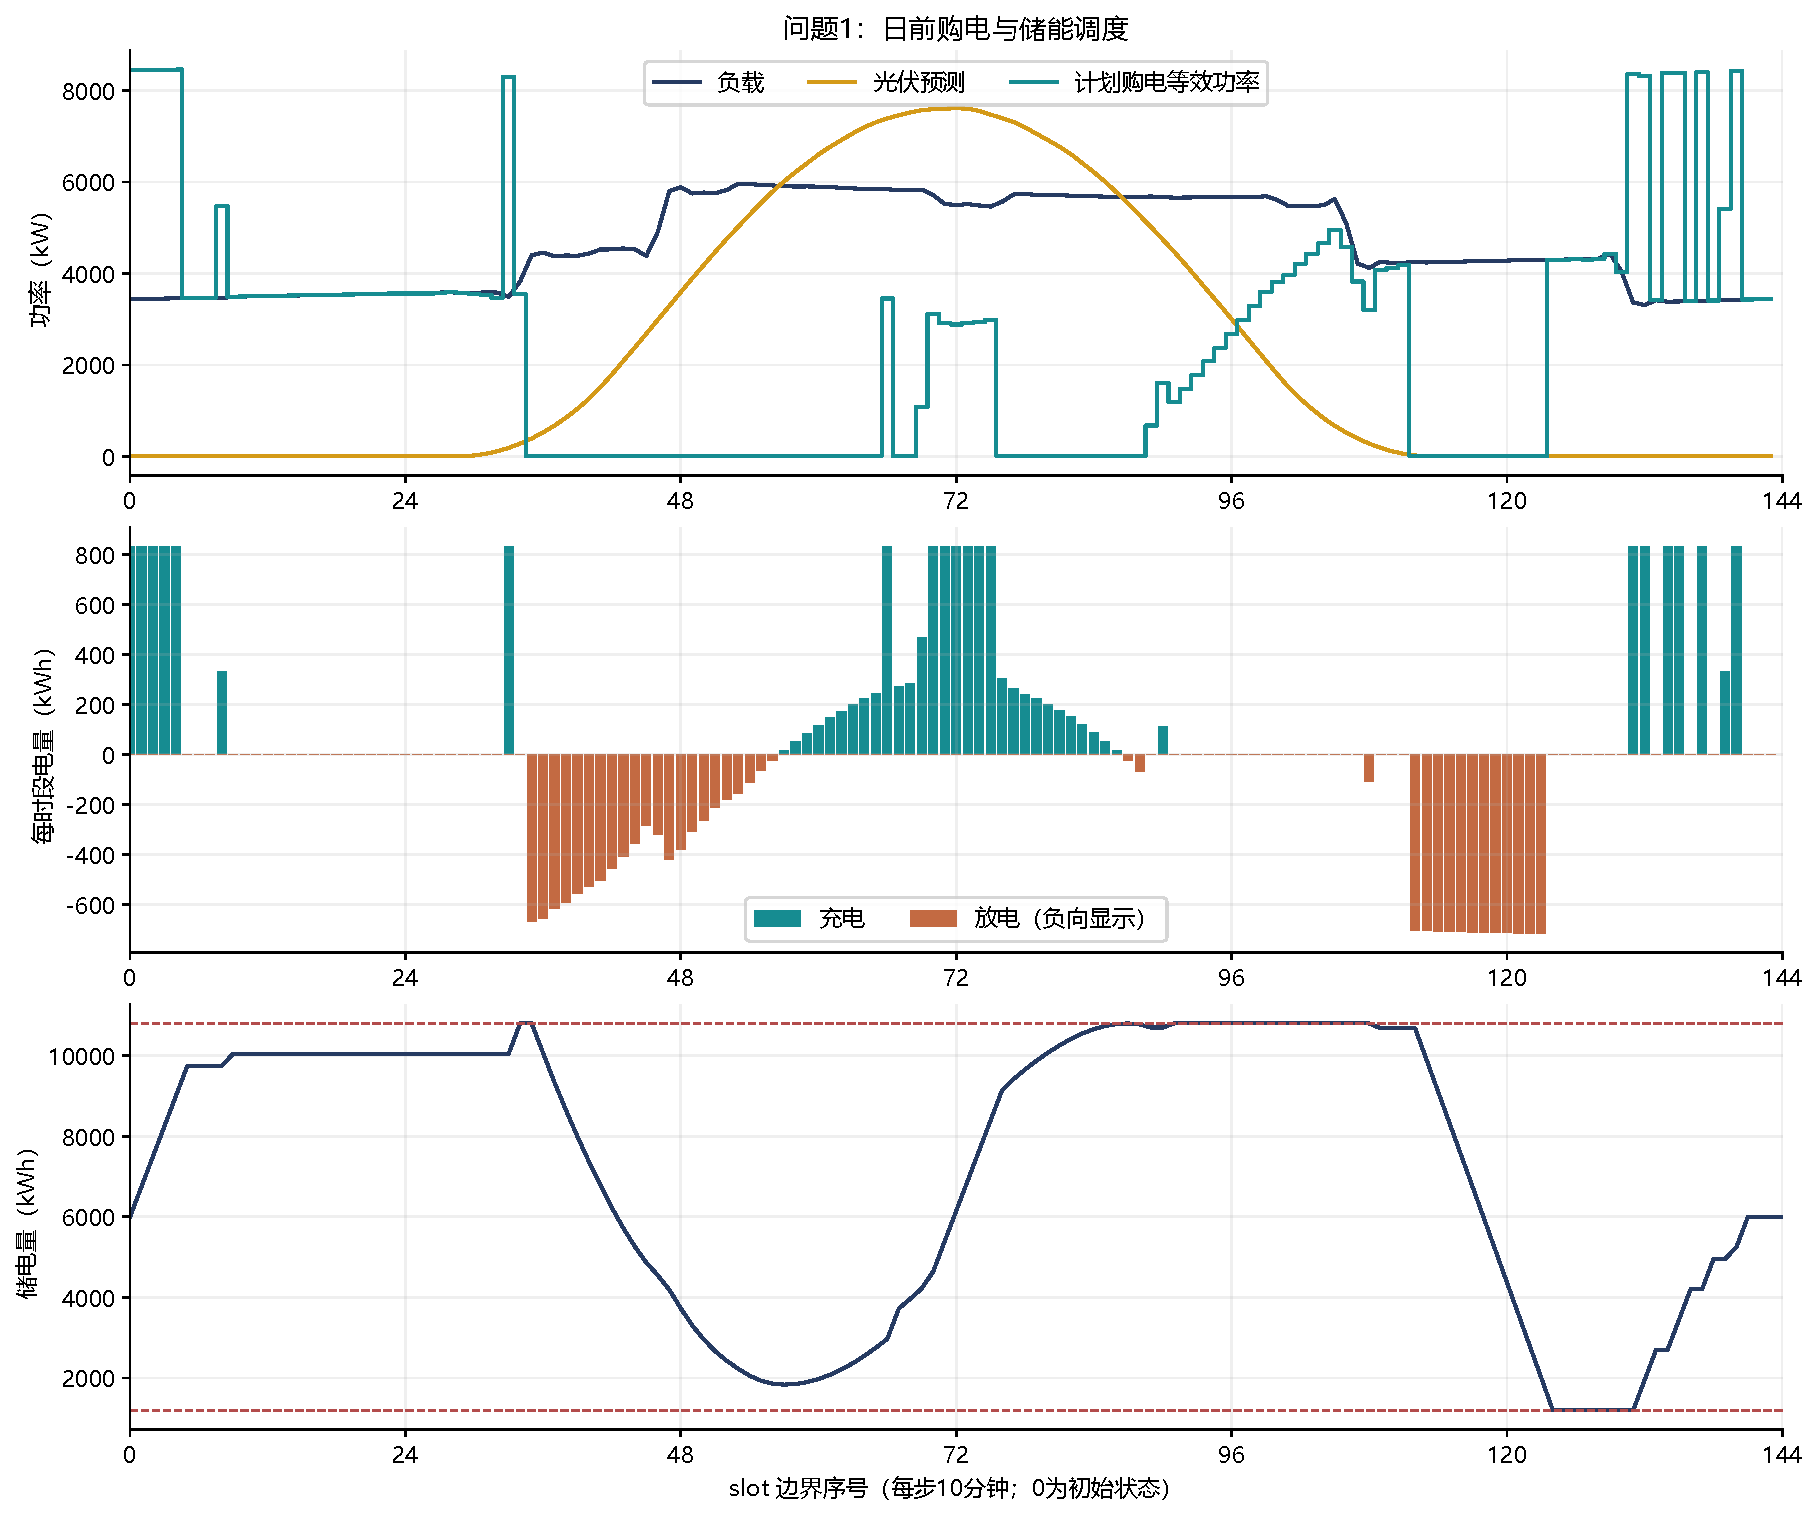
\includegraphics[width=.94\textwidth]{figures/q1_dispatch.pdf}
\caption{问题一的购电、光伏与储能调度；横轴按原始记录位置绘制}\end{figure}
\subsection{经济性与能量守恒}
无储能基准逐段购入正净负荷，购电量61789.9354 kWh，费用48052.0466元。储能优化使费用减少12925.0980元，降幅26.8981\%。该收益同时包含价格时移和光伏消纳改善，并非只来源于峰谷套利。
对状态转移求和，周期边界给出$\sum D_t=0.81\sum C_t$。逐段供需平衡求和后，外网购电等于净负荷加储能损耗及供能富余。当前重算解满足设备容量、功率、边界和能量平衡，且没有超过$10^{-6}$ kWh阈值的同时充放电。该检验支持本算例的物理可行性，不能代替任意参数下的互斥约束证明。
\FloatBarrier

\section{问题二：历史场景下的日前随机规划}
\subsection{场景构造与决策机制}
目标日$d$在0:00尚不知道实际净负荷，选择前31天整日曲线形成$\mathcal S_d=\{d-31,\ldots,d-1\}$，令$N_{d,t}^{(s)}=N_{s,t}$、$\pi_s=1/31$。同一天负载与光伏保持配对，不单独打乱，以保留历史联合变化。等权样本平均近似把未知分布下的期望费用转化为有限场景优化。

第一阶段的$G_t,C_t,D_t,E_t$在场景间共享，当日0:00一并确定；第二阶段的紧急购电$U_t^{(s)}$与富余$W_t^{(s)}$随场景变化。场景约束为
\begin{equation}G_t+D_t-C_t+U_t^{(s)}-W_t^{(s)}=N_{d,t}^{(s)}.\end{equation}
结合共同储能约束，目标为
\begin{equation}\min J_d=\sum_tp_tG_t+\sum_s\pi_s\sum_t5p_tU_t^{(s)}+\varepsilon\sum_t(C_t+D_t).\end{equation}
程序保留显式富余变量，构造稀疏场景平衡等式。一天的储能计划也在场景间共享，因此模型不会在事后为每个真实场景另选一套储能轨迹。

固定充放电、忽略购电非负边界并假设单段净需求$X$连续时，$pG+5p\mathbb E[(X-G)^+]$的一阶条件给出$\Pr(X\leq G)=0.8$。五倍紧急电价因此使计划偏向较高需求分位；实际离散场景和跨段储能约束下，不能用逐段80\%分位曲线替代联合随机规划。

\subsection{实际结算与日际边界}
计划冻结后，定义$B_t=G_t+D_t-C_t$，实际紧急购电为$U_t^{\rm act}=[N_{d,t}-B_t]^+$，供能富余为$W_t^{\rm act}=[B_t-N_{d,t}]^+$。实际费用和总外网购电量分别为
\begin{equation}F_d=\sum_tp_tG_t+\sum_t5p_tU_t^{\rm act},\qquad Q_d=\sum_t(G_t+U_t^{\rm act}).\end{equation}
计划富余不退费，紧急电量不再重复计收普通价格。日前场景期望与事后真实费用分别统计。每日固定6000 kWh边界使日际SOC连续，但不等同于允许跨日储能的全年联合优化。
\subsection{指定日期结果}
所有电量单位为kWh，费用单位为元，保留四位小数，总量使用未舍入值计算。指定十分钟区间按模板标签查询，时间口径见前文。
\Needspace{140pt}\begingroup\centering\captionof{table}{问题二：指定时段购电及全天合同费用}\fontsize{9}{11}\selectfont\setlength{\tabcolsep}{2pt}\renewcommand{\arraystretch}{1.13}
\noindent\begin{minipage}{\textwidth}\centering\textbf{2025-03-20}\par\smallskip
\begin{tabularx}{\textwidth}{|Y|Y|Y|Y|Y|Y|}\hline 时间段&购电量&时间段&购电量&时间段&购电量\\\hline
10:00-10:10 & 0.0000 & 12:00-12:10 & 671.0825 & 14:00-14:10 & 0.0000\\\hline
16:00-16:10 & 545.0921 & 18:00-18:10 & 715.8517 & 20:00-20:10 & 0.0000\\\hline
\multicolumn{2}{|c|}{全天合同购电量}&76168.5490&\multicolumn{2}{c|}{全天合同购电费}&46674.5449\\\hline\end{tabularx}\end{minipage}\par\medskip
\noindent\begin{minipage}{\textwidth}\centering\textbf{2025-06-21}\par\smallskip
\begin{tabularx}{\textwidth}{|Y|Y|Y|Y|Y|Y|}\hline 时间段&购电量&时间段&购电量&时间段&购电量\\\hline
10:00-10:10 & 0.0000 & 12:00-12:10 & 735.1763 & 14:00-14:10 & 0.0000\\\hline
16:00-16:10 & 524.8433 & 18:00-18:10 & 701.5525 & 20:00-20:10 & 54.8683\\\hline
\multicolumn{2}{|c|}{全天合同购电量}&77037.5426&\multicolumn{2}{c|}{全天合同购电费}&47515.1797\\\hline\end{tabularx}\end{minipage}\par\medskip
\noindent\begin{minipage}{\textwidth}\centering\textbf{2025-09-23}\par\smallskip
\begin{tabularx}{\textwidth}{|Y|Y|Y|Y|Y|Y|}\hline 时间段&购电量&时间段&购电量&时间段&购电量\\\hline
10:00-10:10 & 0.0000 & 12:00-12:10 & 494.2704 & 14:00-14:10 & 0.0000\\\hline
16:00-16:10 & 457.1233 & 18:00-18:10 & 802.0687 & 20:00-20:10 & 15.4100\\\hline
\multicolumn{2}{|c|}{全天合同购电量}&68894.1195&\multicolumn{2}{c|}{全天合同购电费}&42711.4056\\\hline\end{tabularx}\end{minipage}\par\medskip
\noindent\begin{minipage}{\textwidth}\centering\textbf{2025-12-21}\par\smallskip
\begin{tabularx}{\textwidth}{|Y|Y|Y|Y|Y|Y|}\hline 时间段&购电量&时间段&购电量&时间段&购电量\\\hline
10:00-10:10 & 0.0000 & 12:00-12:10 & 910.9646 & 14:00-14:10 & 0.0000\\\hline
16:00-16:10 & 778.8025 & 18:00-18:10 & 727.5967 & 20:00-20:10 & 0.0000\\\hline
\multicolumn{2}{|c|}{全天合同购电量}&93392.7439&\multicolumn{2}{c|}{全天合同购电费}&59540.3374\\\hline\end{tabularx}\end{minipage}\par\medskip
\raggedright 注：购电量为日前计划，合同费用不含紧急购电费。\par\endgroup\medskip
\Needspace{140pt}\begingroup\centering\captionof{table}{问题二：指定时段储能充放电及首末储电量}\fontsize{9}{11}\selectfont\setlength{\tabcolsep}{2pt}\renewcommand{\arraystretch}{1.12}
\noindent\begin{minipage}{\textwidth}\centering\textbf{2025-03-20}\par\smallskip\begin{tabularx}{\textwidth}{|Y|Y|Y|Y|Y|Y|}\hline 时间段&充电量&放电量&时间段&充电量&放电量\\\hline
0:00-4:00 & 4500.0000 & 0.0000 & 4:00-8:00 & 1666.6667 & 4769.4828\\\hline
8:00-12:00 & 5850.7628 & 4545.5172 & 12:00-16:00 & 5942.7899 & 912.7777\\\hline
16:00-20:00 & 0.0000 & 5711.4658 & 20:00-24:00 & 5333.3333 & 2928.5342\\\hline
\multicolumn{2}{|c|}{0:00储电量}&6000.0000&\multicolumn{2}{c|}{24:00储电量}&6000.0000\\\hline\end{tabularx}\end{minipage}\par\medskip
\noindent\begin{minipage}{\textwidth}\centering\textbf{2025-06-21}\par\smallskip\begin{tabularx}{\textwidth}{|Y|Y|Y|Y|Y|Y|}\hline 时间段&充电量&放电量&时间段&充电量&放电量\\\hline
0:00-4:00 & 4500.0000 & 0.0000 & 4:00-8:00 & 833.3333 & 5013.6582\\\hline
8:00-12:00 & 5866.5994 & 3113.2873 & 12:00-16:00 & 5833.3333 & 1350.0000\\\hline
16:00-20:00 & 0.0000 & 5833.3333 & 20:00-24:00 & 5333.3333 & 2806.6667\\\hline
\multicolumn{2}{|c|}{0:00储电量}&6000.0000&\multicolumn{2}{c|}{24:00储电量}&6000.0000\\\hline\end{tabularx}\end{minipage}\par\medskip
\noindent\begin{minipage}{\textwidth}\centering\textbf{2025-09-23}\par\smallskip\begin{tabularx}{\textwidth}{|Y|Y|Y|Y|Y|Y|}\hline 时间段&充电量&放电量&时间段&充电量&放电量\\\hline
0:00-4:00 & 4500.0000 & 0.0000 & 4:00-8:00 & 833.3333 & 6618.1059\\\hline
8:00-12:00 & 5947.7825 & 2021.8941 & 12:00-16:00 & 5015.7706 & 240.4780\\\hline
16:00-20:00 & 0.0000 & 5817.0317 & 20:00-24:00 & 5333.3333 & 2822.9683\\\hline
\multicolumn{2}{|c|}{0:00储电量}&6000.0000&\multicolumn{2}{c|}{24:00储电量}&6000.0000\\\hline\end{tabularx}\end{minipage}\par\medskip
\noindent\begin{minipage}{\textwidth}\centering\textbf{2025-12-21}\par\smallskip\begin{tabularx}{\textwidth}{|Y|Y|Y|Y|Y|Y|}\hline 时间段&充电量&放电量&时间段&充电量&放电量\\\hline
0:00-4:00 & 4500.0000 & 0.0000 & 4:00-8:00 & 1666.6667 & 1508.3333\\\hline
8:00-12:00 & 5833.3333 & 7806.6667 & 12:00-16:00 & 7691.4154 & 2315.0465\\\hline
16:00-20:00 & 0.0000 & 5674.8970 & 20:00-24:00 & 5333.3333 & 2965.1030\\\hline
\multicolumn{2}{|c|}{0:00储电量}&6000.0000&\multicolumn{2}{c|}{24:00储电量}&6000.0000\\\hline\end{tabularx}\end{minipage}\par\medskip
\raggedright 注：四小时内充放电均为正表示不同十分钟时段的累计，不表示同时充放电。\par\endgroup
\begin{table}[H]\centering\caption{问题二：四个指定日期的紧急购电区间}\label{tab:emergency-问题二}\fontsize{9}{11}\selectfont\setlength{\tabcolsep}{2pt}\begin{tabular}{|lr|lr|lr|lr|}\hline
\multicolumn{2}{|c|}{2025-03-20} & \multicolumn{2}{|c|}{2025-06-21} & \multicolumn{2}{|c|}{2025-09-23} & \multicolumn{2}{|c|}{2025-12-21}\\\hline
时间段&购电量&时间段&购电量&时间段&购电量&时间段&购电量\\\hline
0:30-0:50 & 37.4563 & 无 & 0.0000 & 2:10-2:20 & 0.8426 & 0:10-0:20 & 3.3265\\
1:20-1:30 & 11.5129 &  &  & 6:10-8:10 & 495.2568 & 1:10-1:30 & 22.4663\\
18:10-18:30 & 8.8068 &  &  & 8:30-8:50 & 24.6687 & 1:40-1:50 & 1.5754\\
18:50-19:20 & 65.2284 &  &  & 9:30-11:20 & 524.1127 & 2:20-2:30 & 6.5004\\
20:10-20:30 & 50.9767 &  &  & 14:30-15:40 & 352.7184 & 3:10-3:30 & 59.6043\\
21:30-21:40 & 8.8117 &  &  & 16:00-18:00 & 370.6423 & 3:40-4:00 & 98.1948\\
23:40-23:50 & 24.6080 &  &  & 19:30-19:40 & 0.7850 & 4:20-4:30 & 0.1398\\
 &  &  &  & 20:20-20:40 & 12.0614 & 5:10-5:30 & 9.6256\\
 &  &  &  & 21:00-21:10 & 9.3900 & 5:40-6:10 & 47.7728\\
 &  &  &  & 22:30-22:40 & 16.1867 & 6:20-6:40 & 25.1715\\
 &  &  &  &  &  & 7:0-7:20 & 10.0867\\
 &  &  &  &  &  & 7:50-8:10 & 24.5775\\
 &  &  &  &  &  & 8:30-8:50 & 39.6960\\
 &  &  &  &  &  & 9:00-9:20 & 26.6807\\
 &  &  &  &  &  & 9:40-10:00 & 42.5371\\
 &  &  &  &  &  & 10:20-12:00 & 1061.3883\\
 &  &  &  &  &  & 12:10-12:30 & 25.4431\\
 &  &  &  &  &  & 12:40-13:30 & 166.5758\\
 &  &  &  &  &  & 14:50-16:10 & 180.2714\\
 &  &  &  &  &  & 16:30-16:40 & 9.4271\\
 &  &  &  &  &  & 17:30-17:40 & 17.9450\\
 &  &  &  &  &  & 18:20-18:30 & 6.9191\\
 &  &  &  &  &  & 18:40-19:10 & 29.1800\\
 &  &  &  &  &  & 19:30-19:40 & 1.0733\\
 &  &  &  &  &  & 19:50-20:20 & 69.4854\\
 &  &  &  &  &  & 22:00-22:10 & 15.0150\\
 &  &  &  &  &  & 23:00-23:20 & 15.7499\\
 &  &  &  &  &  & 23:50-0:00+1 & 6.6598\\
\hline\end{tabular}\end{table}

\begin{table}[H]\centering\small
\caption{问题二：实际总购电与费用}
\begin{tabular}{lrrrr}\toprule
日期 & 实际购电量 & 紧急购电量 & 紧急费用 & 实际总费用\\\midrule
2025-03-20 & 76375.9499 & 207.4009 & 1030.6857 & 47705.2306\\
2025-06-21 & 77037.5426 & 0.0000 & 0.0000 & 47515.1797\\
2025-09-23 & 70700.7840 & 1806.6645 & 7617.1530 & 50328.5586\\
2025-12-21 & 95415.8327 & 2023.0888 & 6853.4988 & 66393.8362\\
\bottomrule\end{tabular}\end{table}
\FloatBarrier
\subsection{全期结果与风险解释}

\begin{table}[H]\centering\small
\caption{问题二：334天结果汇总}
\begin{tabular}{lr}\toprule
指标 & 数值\\\midrule
计划购电量/kWh & 25433452.3036\\
紧急购电量/kWh & 477446.0574\\
实际总购电量/kWh & 25910898.3610\\
计划费/元 & 15771812.6875\\
紧急费/元 & 1837978.9991\\
实际总费用/元 & 17609791.6865\\
发生紧急购电天数 & 249\\
\bottomrule\end{tabular}\end{table}
紧急电量占比为1.8426\%，费用占比却为10.4373\%，反映惩罚倍率和缺口时刻电价的共同作用。249天发生补购，低紧急电量占比不表示低事件频率。6月21日没有补购，但该月整体风险仍可能较高，单个指定日期不能代表整月。

\begin{figure}[H]\centering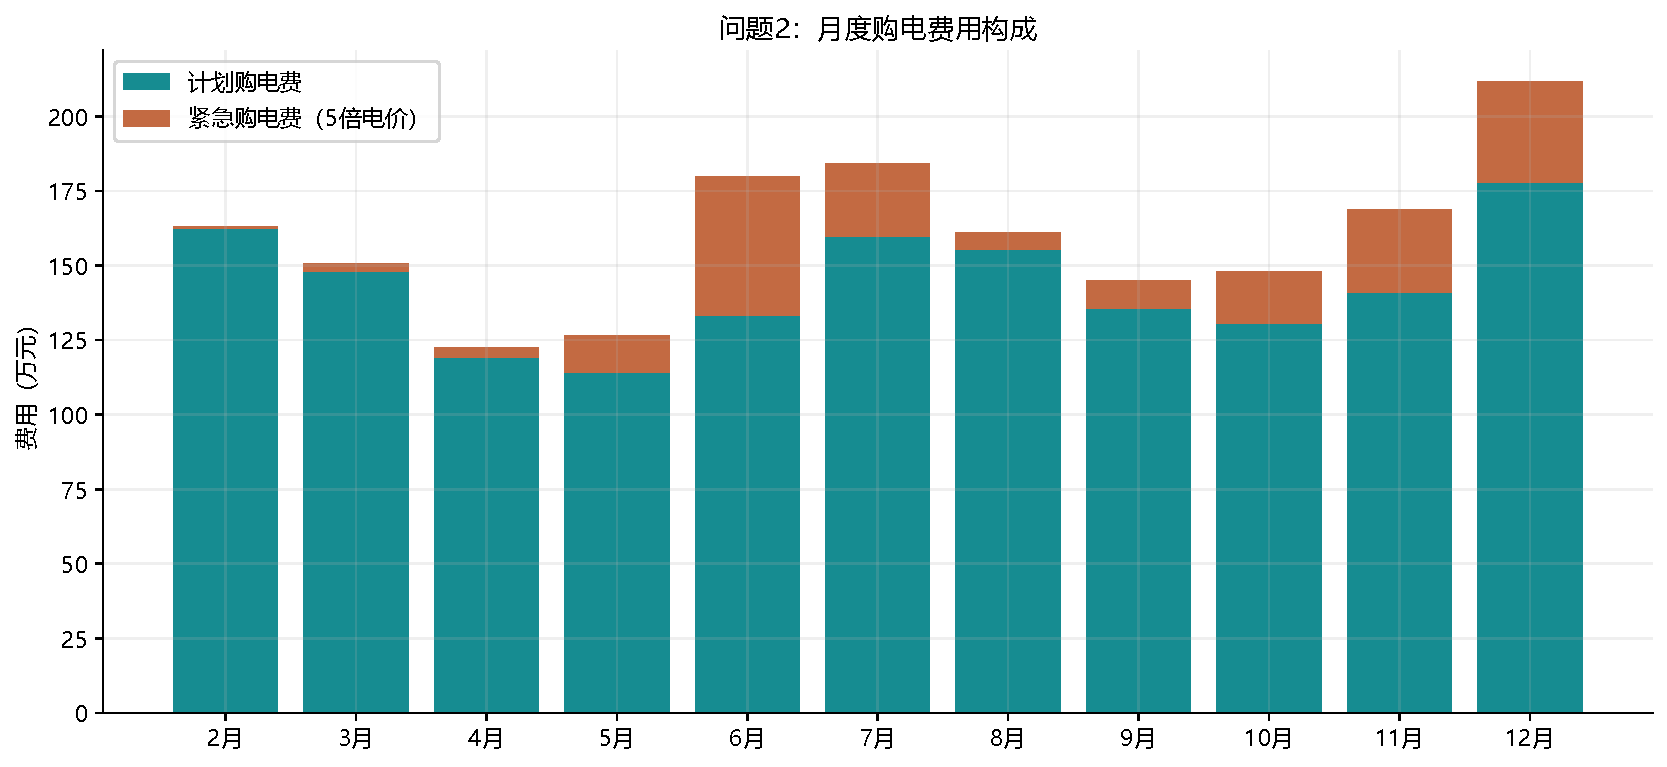
\includegraphics[width=.94\textwidth]{figures/q2_monthly.pdf}
\caption{问题二的月度计划费用与紧急费用}\end{figure}
风险来自历史场景对当前净负荷的覆盖不足。增加备购可以减少紧急费用，却可能扩大已支付合同的供能富余，因此需要联合权衡。与确定性均值、分位数及风险规避方法的同信息对照见后文，不能仅凭本模型可行就宣称其实际费用在所有策略中最低。
\FloatBarrier

\section{问题三：预报更新下的滚动随机规划}
\subsection{建模思路与信息边界}
问题三在问题二的日前计划基础上，增加了光伏预报更新与购电合同调整机制。本文将31天历史场景与滚动时域优化结合：0:00利用最新光伏预报制定全天计划；6:00、12:00等更新时刻重新构造剩余时段的净负荷场景，在已执行储能状态和已确认合同的基础上调整未来策略。实际净负荷超出计划净供能的部分，仍由五倍电价紧急购电补足。

将一天按记录顺序划分为144个十分钟时段，$\Delta t=1/6\,\mathrm h$；内部索引$t=1,\ldots,144$，预报时刻$r\in\{0,6,12,18\}$对应已完成时段数$\tau_r=6r$。设$\mathcal T_r=\{\tau_r+1,\ldots,144\}$。每次优化只使用前31天的历史实际数据、当次已发布预报，以及发布前最后一个已完成时段的观测值。目标日未来实际负载和光伏仅用于事后评价，不进入当次决策。

本文延续问题二每日首末储电量为6000 kWh的周期边界，只使用预报中截至当日24:00的部分。日内更新时，初始储电量必须承接已经执行的充放电结果，不能在6:00或12:00重新设为6000 kWh。该边界有利于比较不同预报组合，但限制了跨日储能和次日预报信息的利用。

\subsection{光伏预报插值及净负荷场景}
附件3按每天四个发布时间给出未来24小时整点预报。设$\widehat P_{d,r,h}$为第$d$日$r$时发布的第$h$小时光伏功率预报，令$y_0$为当前已观测光伏功率，$y_h=\widehat P_{d,r,h}$。0:00锚点取零，其他时刻使用发布前最后一条实际记录。对相邻整点间的$x\in[h,h+1]$，线性插值为
\begin{equation}
\widetilde P_{d,r}(x)=(h+1-x)y_h+(x-h)y_{h+1}.
\end{equation}
本文在十分钟区间中点采样，$\widehat P^{10}_{d,r,t}=\widetilde P_{d,r}((t-\tau_r-1/2)\Delta t)$。历史预测误差采用相同插值方式计算，保证场景、优化和误差评价口径一致。

对历史日期$s\in\mathcal S_d=\{d-31,\ldots,d-1\}$，按相同发布时间和插值方法计算光伏预测误差，并与同一天负载配对：
\begin{align}
e_{s,r,t}&=P^{\mathrm{PV}}_{s,t}-\widehat P^{10}_{s,r,t},\\
P^{\mathrm{PV},(s)}_{d,r,t}&=\max\{0,\widehat P^{10}_{d,r,t}+e_{s,r,t}\},\\
N^{(s)}_{d,r,t}&=\bigl(P^{\mathrm L}_{s,t}-P^{\mathrm{PV},(s)}_{d,r,t}\bigr)\Delta t,
\qquad \pi_s=1/31.\label{eq:p3-scenario}
\end{align}
式\eqref{eq:p3-scenario}以目标日新预报为中心，叠加近期历史误差，避免将预报视为确定值；非负截断避免出现负光伏功率。负载不另行拟合预测模型，同日负载与光伏误差的配对保留历史联合变化。其适用前提是近期误差具有一定可迁移性，尚不能保证极端天气或负载突变均被31个场景覆盖。

\subsection{初始计划与逐次调整结算}
记$G^0_t$为0:00初始合同购电量；日内更新前后的合同量分别为$G^{\mathrm{old}}_t$和$G^{\mathrm{new}}_t$。定义增购量$A^r_t$和削减量$B^r_t$，则
\begin{equation}
G^{\mathrm{new}}_t=G^{\mathrm{old}}_t+A^r_t-B^r_t,
\qquad A^r_t\geq0,\quad 0\leq B^r_t\leq G^{\mathrm{old}}_t.
\label{eq:p3-contract}
\end{equation}
本文将题面50\%违约电价解释为取消电量仅退回原价的50\%，被取消部分承担其余50\%损失。每次调整相对于上一版已确认合同结算，其净费用为
\begin{equation}
K_d^r=\sum_{t\in\mathcal T_r}p_t(1.5A^r_t-0.5B^r_t).
\label{eq:p3-cash}
\end{equation}
例如原计划100 kWh削减为80 kWh，初始支付$100p$，获得$10p$退款，最终支出$90p$；若增至120 kWh，则支付$100p+1.5p\times20=130p$。因此调整净费用可以为负，不能将退款误记为负违约损失，也不能在保留全部初始费用的同时再次对被取消电量重复收费。此处采用交付时段对应的分时电价$p_t$；逐次结算和退款解释均为本文统一的交易口径。

相同时段若同时增购和削减相同电量，会增加$p_t$倍该电量的费用而不改变合同。因此，正电价下同时增减没有经济优势。多次调整的路径仍影响结算，不能只用最终合同与初始合同之差代替每次交易。

\subsection{随机线性规划及滚动执行}
设$C_t,D_t,E_t$分别为充电输入电量、放电输出电量和时段末储电量，$U^{(s)}_t$为场景紧急购电量。0:00的目标为
\begin{equation}
\min\ \sum_{t=1}^{144}p_tG^0_t
+\frac1{31}\sum_{s\in\mathcal S_d}\sum_{t=1}^{144}5p_tU^{(s)}_t
+\varepsilon\sum_{t=1}^{144}(C_t+D_t),\quad\varepsilon=10^{-8}.
\label{eq:p3-init}
\end{equation}
在$r>0$时，已支付合同费用及过去费用为沉没成本，剩余时域的优化目标改为
\begin{equation}
\min\ \sum_{t\in\mathcal T_r}p_t(1.5A^r_t-0.5B^r_t)
+\frac1{31}\sum_s\sum_{t\in\mathcal T_r}5p_tU^{(s)}_t
+\varepsilon\sum_{t\in\mathcal T_r}(C_t+D_t).
\label{eq:p3-roll}
\end{equation}
各阶段满足共同的设备与场景约束：
\begin{align}
U^{(s)}_t&\geq N^{(s)}_{d,r,t}-G_t-D_t+C_t,\qquad U^{(s)}_t\geq0,\\
E_t&=E_{t-1}+0.9C_t-D_t/0.9,\\
1200&\leq E_t\leq10800,\qquad 0\leq C_t,D_t\leq5000\Delta t,\\
G_t&\geq0,\qquad E_{144}=6000,\\
E_{\tau_r}&=E^{\mathrm{exec}}_{\tau_r}.\label{eq:p3-boundary}
\end{align}
0:00取$E^{\mathrm{exec}}_0=6000$，调整阶段另加入式\eqref{eq:p3-contract}。上述不等式等价于在场景电量平衡中引入非负供能富余量后将其消去。每个阶段的合同与充放电变量在31个场景间共享，紧急购电变量随场景变化。目标中的小惩罚仅用于减少不必要的吞吐；报告费用剔除数值辅助惩罚。

求解器显式保留场景供能富余变量，以稀疏等式矩阵调用HiGHS；正文中的正缺口不等式是等价数学表述。对所选预报集合$\mathcal R=\{0,6,12\}$，实际执行遵循
\begin{equation}
\underbrace{\text{0点求解全天}}_{\text{执行0至6点}}
\longrightarrow
\underbrace{\text{6点重算余下18小时}}_{\text{执行6至12点}}
\longrightarrow
\underbrace{\text{12点重算余下12小时}}_{\text{执行12至24点}}.
\end{equation}
每次只冻结执行到下一个更新时刻的结果，未执行部分可以调整，式\eqref{eq:p3-boundary}保证储能状态连续。该方法是滚动求解一系列两阶段随机规划，并未建立包含未来预报分支的完整多阶段场景树，因此单次LP最优不等于全年实际费用全局最优。

\subsection{实际费用与合同量的区分}
将各阶段执行片段拼接为$G^{\rm exec},C^{\rm exec},D^{\rm exec}$，实际缺口为
\begin{equation}U_{d,t}^{\rm act}=[N_{d,t}-G_{d,t}^{\rm exec}-D_{d,t}^{\rm exec}+C_{d,t}^{\rm exec}]^+.\end{equation}
日费用为$F_d=\sum_tp_tG_{d,t}^0+\sum_rK_d^r+\sum_t5p_tU_{d,t}^{\rm act}$。实际总外网购电量为$\sum_t(G_{d,t}^{\rm exec}+U_{d,t}^{\rm act})$，与初始合同总量、执行合同总量不同。各更新阶段以相同交付时段电价结算，逐次退款不等于仅对最终与初始合同的差额结算。
\subsection{指定日期结果}
所有电量单位为kWh，费用单位为元，保留四位小数，总量使用未舍入值计算。指定十分钟区间按模板标签查询，时间口径见前文。
\Needspace{140pt}\begingroup\centering\captionof{table}{问题三：指定时段购电及全天合同费用}\fontsize{9}{11}\selectfont\setlength{\tabcolsep}{2pt}\renewcommand{\arraystretch}{1.13}
\noindent\begin{minipage}{\textwidth}\centering\textbf{2025-03-20}\par\smallskip
\begin{tabularx}{\textwidth}{|Y|Y|Y|Y|Y|Y|}\hline 时间段&购电量&时间段&购电量&时间段&购电量\\\hline
10:00-10:10 & \shortstack{0.0000\\0.0000} & 12:00-12:10 & \shortstack{599.0619\\521.3555} & 14:00-14:10 & \shortstack{0.0000\\0.0000}\\\hline
16:00-16:10 & \shortstack{646.6018\\493.7743} & 18:00-18:10 & \shortstack{711.7617\\711.7617} & 20:00-20:10 & \shortstack{0.0000\\0.0000}\\\hline
\multicolumn{2}{|c|}{全天合同购电量}&\shortstack{73413.4543\\68090.0668}&\multicolumn{2}{c|}{全天合同购电费}&\shortstack{44712.5869\\43432.6403}\\\hline\end{tabularx}\end{minipage}\par\medskip
\noindent\begin{minipage}{\textwidth}\centering\textbf{2025-06-21}\par\smallskip
\begin{tabularx}{\textwidth}{|Y|Y|Y|Y|Y|Y|}\hline 时间段&购电量&时间段&购电量&时间段&购电量\\\hline
10:00-10:10 & \shortstack{0.0000\\0.0000} & 12:00-12:10 & \shortstack{561.4173\\561.4173} & 14:00-14:10 & \shortstack{0.0000\\0.0000}\\\hline
16:00-16:10 & \shortstack{575.5241\\575.5241} & 18:00-18:10 & \shortstack{686.7649\\686.7649} & 20:00-20:10 & \shortstack{54.8683\\54.8683}\\\hline
\multicolumn{2}{|c|}{全天合同购电量}&\shortstack{74343.0580\\74194.0088}&\multicolumn{2}{c|}{全天合同购电费}&\shortstack{45952.6560\\46011.6473}\\\hline\end{tabularx}\end{minipage}\par\medskip
\noindent\begin{minipage}{\textwidth}\centering\textbf{2025-09-23}\par\smallskip
\begin{tabularx}{\textwidth}{|Y|Y|Y|Y|Y|Y|}\hline 时间段&购电量&时间段&购电量&时间段&购电量\\\hline
10:00-10:10 & \shortstack{0.0000\\0.0000} & 12:00-12:10 & \shortstack{445.1351\\430.5782} & 14:00-14:10 & \shortstack{0.0000\\0.0000}\\\hline
16:00-16:10 & \shortstack{600.6055\\563.8344} & 18:00-18:10 & \shortstack{833.5750\\833.5750} & 20:00-20:10 & \shortstack{15.4100\\15.4100}\\\hline
\multicolumn{2}{|c|}{全天合同购电量}&\shortstack{76400.1981\\74670.4428}&\multicolumn{2}{c|}{全天合同购电费}&\shortstack{47983.4554\\47448.1926}\\\hline\end{tabularx}\end{minipage}\par\medskip
\noindent\begin{minipage}{\textwidth}\centering\textbf{2025-12-21}\par\smallskip
\begin{tabularx}{\textwidth}{|Y|Y|Y|Y|Y|Y|}\hline 时间段&购电量&时间段&购电量&时间段&购电量\\\hline
10:00-10:10 & \shortstack{0.0000\\0.0000} & 12:00-12:10 & \shortstack{972.1554\\866.2299} & 14:00-14:10 & \shortstack{0.0000\\0.0000}\\\hline
16:00-16:10 & \shortstack{825.5984\\825.5984} & 18:00-18:10 & \shortstack{727.5967\\727.5967} & 20:00-20:10 & \shortstack{0.0000\\0.0000}\\\hline
\multicolumn{2}{|c|}{全天合同购电量}&\shortstack{95529.3993\\94748.8343}&\multicolumn{2}{c|}{全天合同购电费}&\shortstack{61023.2426\\61000.9854}\\\hline\end{tabularx}\end{minipage}\par\medskip
\raggedright 注：每格上行为0:00计划，下行为执行合同；下行合同费用为初始计划费加逐次调整净费。\par\endgroup\medskip
\Needspace{140pt}\begingroup\centering\captionof{table}{问题三：指定时段储能充放电及首末储电量}\fontsize{9}{11}\selectfont\setlength{\tabcolsep}{2pt}\renewcommand{\arraystretch}{1.12}
\noindent\begin{minipage}{\textwidth}\centering\textbf{2025-03-20}\par\smallskip\begin{tabularx}{\textwidth}{|Y|Y|Y|Y|Y|Y|}\hline 时间段&充电量&放电量&时间段&充电量&放电量\\\hline
0:00-4:00 & 4500.0000 & 0.0000 & 4:00-8:00 & 833.3333 & 6024.2476\\\hline
8:00-12:00 & 5515.1627 & 2615.7524 & 12:00-16:00 & 5453.3594 & 249.7318\\\hline
16:00-20:00 & 21.2974 & 5726.9239 & 20:00-24:00 & 5333.3333 & 2925.0981\\\hline
\multicolumn{2}{|c|}{0:00储电量}&6000.0000&\multicolumn{2}{c|}{24:00储电量}&6000.0000\\\hline\end{tabularx}\end{minipage}\par\medskip
\noindent\begin{minipage}{\textwidth}\centering\textbf{2025-06-21}\par\smallskip\begin{tabularx}{\textwidth}{|Y|Y|Y|Y|Y|Y|}\hline 时间段&充电量&放电量&时间段&充电量&放电量\\\hline
0:00-4:00 & 4500.0000 & 0.0000 & 4:00-8:00 & 833.3333 & 4597.3706\\\hline
8:00-12:00 & 5605.0111 & 3272.8270 & 12:00-16:00 & 5231.8329 & 1092.5664\\\hline
16:00-20:00 & 228.2967 & 5834.6120 & 20:00-24:00 & 5333.3333 & 2805.3880\\\hline
\multicolumn{2}{|c|}{0:00储电量}&6000.0000&\multicolumn{2}{c|}{24:00储电量}&6000.0000\\\hline\end{tabularx}\end{minipage}\par\medskip
\noindent\begin{minipage}{\textwidth}\centering\textbf{2025-09-23}\par\smallskip\begin{tabularx}{\textwidth}{|Y|Y|Y|Y|Y|Y|}\hline 时间段&充电量&放电量&时间段&充电量&放电量\\\hline
0:00-4:00 & 4500.0000 & 0.0000 & 4:00-8:00 & 833.3333 & 6086.0836\\\hline
8:00-12:00 & 5893.1650 & 2517.5563 & 12:00-16:00 & 5662.2298 & 756.2298\\\hline
16:00-20:00 & 0.0000 & 5817.0317 & 20:00-24:00 & 5333.3333 & 2822.9683\\\hline
\multicolumn{2}{|c|}{0:00储电量}&6000.0000&\multicolumn{2}{c|}{24:00储电量}&6000.0000\\\hline\end{tabularx}\end{minipage}\par\medskip
\noindent\begin{minipage}{\textwidth}\centering\textbf{2025-12-21}\par\smallskip\begin{tabularx}{\textwidth}{|Y|Y|Y|Y|Y|Y|}\hline 时间段&充电量&放电量&时间段&充电量&放电量\\\hline
0:00-4:00 & 4500.0000 & 0.0000 & 4:00-8:00 & 1656.3466 & 1655.7650\\\hline
8:00-12:00 & 5880.1685 & 7484.9920 & 12:00-16:00 & 7736.9824 & 2581.8781\\\hline
16:00-20:00 & 32.3865 & 5676.3612 & 20:00-24:00 & 5333.3333 & 2963.7697\\\hline
\multicolumn{2}{|c|}{0:00储电量}&6000.0000&\multicolumn{2}{c|}{24:00储电量}&6000.0000\\\hline\end{tabularx}\end{minipage}\par\medskip
\raggedright 注：四小时内充放电均为正表示不同十分钟时段的累计，不表示同时充放电。\par\endgroup
\begin{table}[H]\centering\caption{问题三：四个指定日期的紧急购电区间}\label{tab:emergency-问题三}\fontsize{9}{11}\selectfont\setlength{\tabcolsep}{2pt}\begin{tabular}{|lr|lr|lr|lr|}\hline
\multicolumn{2}{|c|}{2025-03-20} & \multicolumn{2}{|c|}{2025-06-21} & \multicolumn{2}{|c|}{2025-09-23} & \multicolumn{2}{|c|}{2025-12-21}\\\hline
时间段&购电量&时间段&购电量&时间段&购电量&时间段&购电量\\\hline
0:30-0:50 & 37.4563 & 无 & 0.0000 & 2:10-2:20 & 0.8426 & 0:10-0:20 & 3.3265\\
1:20-1:30 & 11.5129 &  &  & 19:30-19:40 & 0.7850 & 1:10-1:30 & 22.4663\\
8:20-8:40 & 32.7797 &  &  & 20:20-20:40 & 12.0614 & 1:40-1:50 & 1.5754\\
8:50-9:30 & 137.5983 &  &  & 21:00-21:10 & 9.3900 & 2:20-2:30 & 6.5004\\
9:50-10:10 & 57.9445 &  &  & 22:30-22:40 & 16.1867 & 3:10-3:30 & 59.6043\\
11:10-12:10 & 345.6128 &  &  &  &  & 3:40-4:00 & 98.1948\\
12:40-13:00 & 150.4760 &  &  &  &  & 4:20-4:30 & 0.1398\\
13:10-13:50 & 148.0535 &  &  &  &  & 5:10-5:30 & 9.6256\\
14:00-14:40 & 31.2403 &  &  &  &  & 5:40-6:10 & 47.7728\\
15:30-16:30 & 96.1899 &  &  &  &  & 6:30-6:40 & 0.4267\\
16:40-17:00 & 3.7317 &  &  &  &  & 8:00-8:10 & 13.3395\\
18:10-18:30 & 8.8068 &  &  &  &  & 8:30-8:40 & 6.0161\\
18:50-19:20 & 68.9363 &  &  &  &  & 9:00-9:10 & 0.7455\\
20:10-20:30 & 53.6129 &  &  &  &  & 9:40-10:10 & 57.4065\\
21:30-21:40 & 8.8117 &  &  &  &  & 10:30-12:30 & 728.2815\\
23:40-23:50 & 24.6080 &  &  &  &  & 12:50-13:20 & 102.9197\\
 &  &  &  &  &  & 14:00-14:10 & 9.0172\\
 &  &  &  &  &  & 17:30-17:40 & 17.9450\\
 &  &  &  &  &  & 18:20-18:30 & 6.9191\\
 &  &  &  &  &  & 18:40-19:10 & 29.1800\\
 &  &  &  &  &  & 19:30-19:40 & 1.0733\\
 &  &  &  &  &  & 19:50-20:20 & 69.4854\\
 &  &  &  &  &  & 22:00-22:10 & 15.0150\\
 &  &  &  &  &  & 23:00-23:20 & 15.7499\\
 &  &  &  &  &  & 23:50-0:00+1 & 6.6598\\
\hline\end{tabular}\end{table}

\begin{table}[H]\centering\small
\caption{问题三：实际总购电与费用}
\begin{tabular}{lrrrr}\toprule
日期 & 实际购电量 & 紧急购电量 & 紧急费用 & 实际总费用\\\midrule
2025-03-20 & 69307.4385 & 1217.3717 & 4610.4730 & 48043.1133\\
2025-06-21 & 74194.0088 & 0.0000 & 0.0000 & 46011.6473\\
2025-09-23 & 74709.7084 & 39.2657 & 166.1880 & 47614.3806\\
2025-12-21 & 96078.2205 & 1329.3861 & 4334.5379 & 65335.5233\\
\bottomrule\end{tabular}\end{table}
\FloatBarrier

\begin{figure}[H]\centering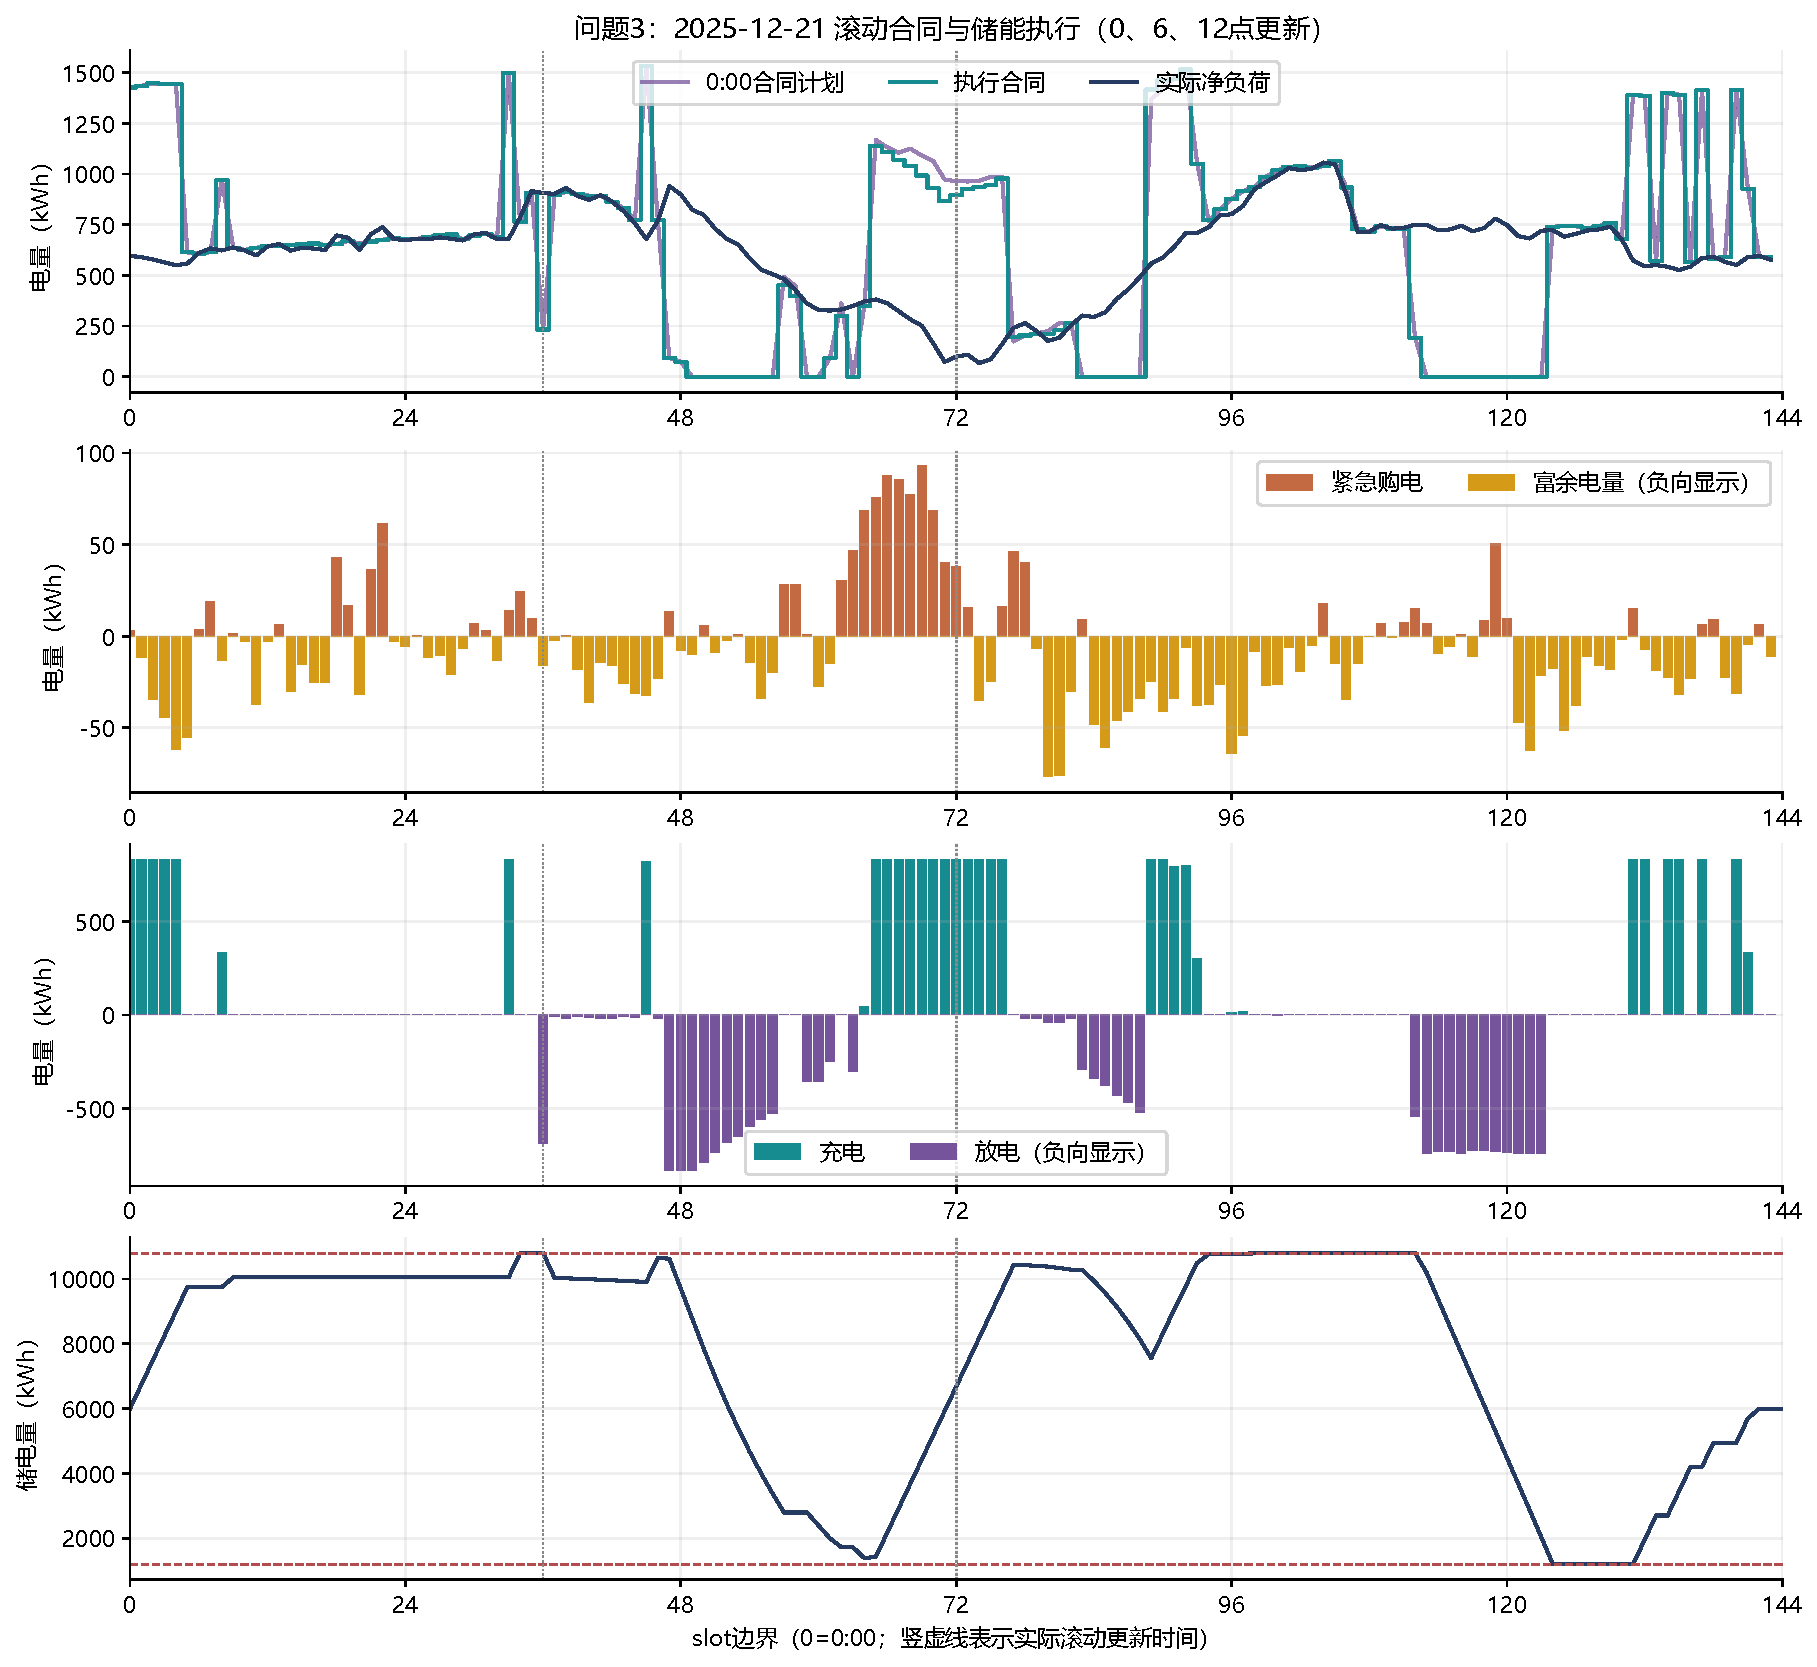
\includegraphics[width=.94\textwidth]{figures/q3_dispatch.pdf}
\caption{12月21日三时刻策略执行轨迹，6点和12点后仅调整未执行部分}\end{figure}
\subsection{预报时刻的经济价值}

\begin{table}[H]\centering\small
\caption{中点插值下六种预报组合的334天回测}
\begin{tabular}{lrrr}\toprule
预报组合 & 总费用/元 & 紧急电量/kWh & 相对仅0点节省/元\\\midrule
0 & 17365850.5168 & 380700.5461 & 0.0000\\
0+6 & 17102438.5627 & 300935.5745 & 263411.9541\\
0+6+12 & 17020306.6465 & 282085.6383 & 345543.8702\\
0+6+12+18 & 17020342.9202 & 282112.5626 & 345507.5965\\
0+12+18 & 17109577.9735 & 321945.8997 & 256272.5433\\
0+6+18 & 17102086.8102 & 300951.5733 & 263763.7066\\
\bottomrule\end{tabular}\end{table}
沿0点、加入6点、再加入12点的顺序，费用分别减少263411.9541元和82131.9161元。进一步加入18点增加36.2737元。由四时刻集合删除6点和12点，分别增加89235.0532元和81743.8900元。因此当前回测支持保留6点、12点。
18点的费用变化相对于全期费用极小，应表述为“本次回测未见额外经济收益”，不应认为18点预报普遍无用。六种组合未穷举所有子集，且策略在同年回测中比较并选择，仍需独立验证期判断泛化效果。
\subsection{共同窗口预测误差与离散稳健性}
用MAE与RMSE评价光伏功率预报，避免夜间真值为零时MAPE失真。不同发布时间的剩余窗口长度不同，不能直接把RMSE下降全部归因于预报更新。固定18:00--24:00共同窗口后，各组均使用12024个样本。

\begin{table}[H]\centering\small
\caption{不同预报的功率误差（kW）}
\begin{tabular}{lrrr}\toprule
发布时间 & 剩余窗口样本数 & 剩余RMSE & 共同窗口RMSE\\\midrule
0:00 & 48096 & 388.7783 & 62.7411\\
6:00 & 36072 & 286.8708 & 60.7876\\
12:00 & 24048 & 166.1577 & 60.5573\\
18:00 & 12024 & 60.0726 & 60.0726\\
\bottomrule\end{tabular}\end{table}
12点到18点在共同窗口的RMSE仅改善0.4847 kW。误差更小不保证合同调整与紧急费用之和更低，经济价值仍需通过完整执行评价。

\begin{figure}[H]\centering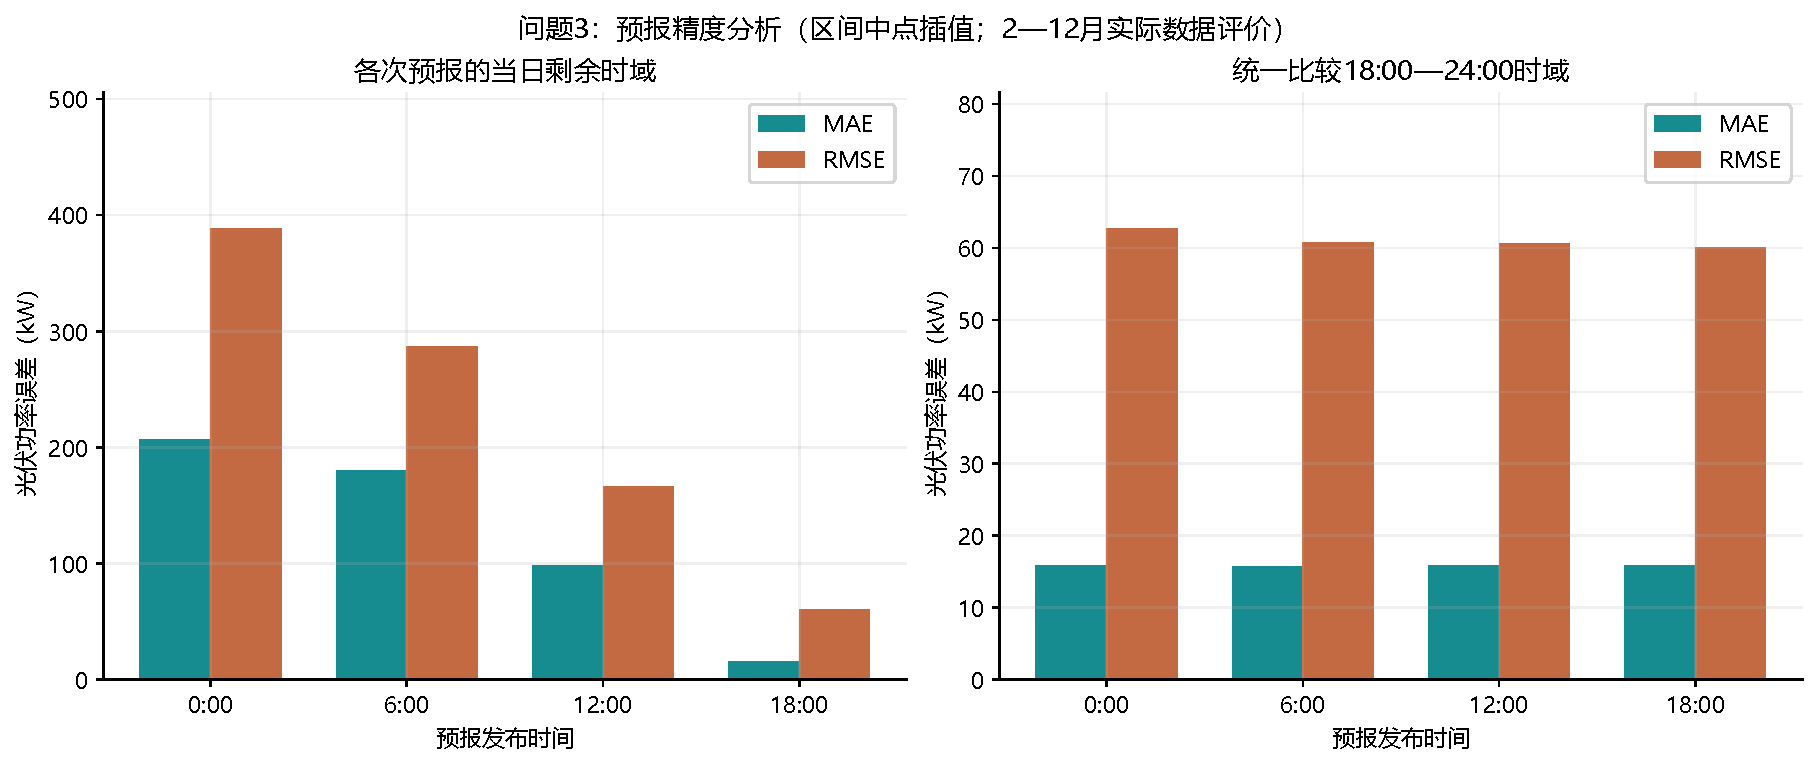
\includegraphics[width=.94\textwidth]{figures/q3_accuracy.pdf}
\caption{预报误差比较：剩余窗口与共同晚间窗口分别统计}\end{figure}
作为离散口径对照，既有端点三时刻实现的费用为17013832.1962元，比中点实现低6474.4504元，约0.0380\%。该差异同时受到采样与数值实现影响，不能证明端点插值普遍更好。两种实现均支持当前三时刻选择；本文主结果、第四问和算法对照统一采用中点实现，端点结果只作为稳健性补充。
\subsection{全期结果与收益分解}

\begin{table}[H]\centering\small
\caption{问题三：334天正式主策略汇总}
\begin{tabular}{lr}\toprule
指标 & 数值\\\midrule
初始合同量/kWh & 25627255.4413\\
执行合同量/kWh & 24999199.3025\\
紧急购电量/kWh & 282085.6383\\
实际总购电量/kWh & 25281284.9407\\
初始计划费/元 & 15933478.6262\\
调整净费/元 & 9377.4177\\
紧急费/元 & 1077450.6027\\
实际总费/元 & 17020306.6465\\
\bottomrule\end{tabular}\end{table}
相对问题二，费用减少589485.0400元，降幅3.3475\%；紧急电量减少40.9178\%。其中由问题二到仅0点预报节省243941.1698元，再引入6点、12点滚动更新节省345543.8702元。这区分了初始预报信息与日内调整的收益，不能把全部差异归因于滚动控制。仍有243天发生紧急补购，说明策略减少费用和补购规模，并未消除预测偏差。
\FloatBarrier

\section{问题四：波动电价下的策略比较}
\subsection{价格信息与模型修正}
将固定分时电价$p_t$推广为目标日期的$p_{d,t}$。附件4价格曲线作为给定条件输入，而负载、光伏仍保持原有信息约束。365天日期与144个时间列严格与附件2对齐；1月价格不计入334天正式结果。若未来价格未知，则需另建预测或随机价格场景，超出当前基础方案。

问题4-2将第二问目标改为$\sum_tp_{d,t}G_t+\sum_s\pi_s\sum_t5p_{d,t}U_t^{(s)}+\varepsilon\sum_t(C_t+D_t)$，其他约束不变。问题4-3同样替换初始计划、紧急补购与调整交易的价格：
\begin{equation}K_d^r=\sum_{t\in\mathcal T_r}p_{d,t}(1.5A_t^r-0.5B_t^r).\end{equation}
历史窗口、中点插值、设备参数及每日边界均保持一致，正式4-3继续采用0、6、12点策略。固定价格基线使用同一策略，避免把更新时间变化混入价格机制比较。
\subsection{年度结果与经济机制}

\begin{table}[H]\centering\small
\caption{固定与波动价格下的334天对比}
\begin{tabular}{lrrr}\toprule
策略 & 总费用/元 & 紧急电量/kWh & 紧急费/元\\\midrule
问题二 & 17609791.6865 & 477446.0574 & 1837978.9991\\
问题4-2 & 17923538.0937 & 476815.3372 & 2115778.9637\\
问题三 & 17020306.6465 & 282085.6383 & 1077450.6027\\
问题4-3 & 17244554.4259 & 281004.2788 & 1214613.7429\\
\bottomrule\end{tabular}\end{table}
波动价格下，日前策略费用增加313746.4071元（1.7817\%），滚动策略增加224247.7793元（1.3175\%）。在相同波动价格环境中，4-3比4-2节省678983.6678元，降幅3.7882\%。该差异体现新增预报、场景构造及滚动交易的综合价值。
两组动态策略的紧急电量略低于固定价格基线，但紧急费用更高，说明缺口出现在哪个价格时段同样重要。平均电价降低也不能保证总费用降低，因为费用取决于购电量与逐时价格的配对及五倍补购。充放电时移还受到0.81往返效率约束；简化的无其他约束套利条件为高价超过低价的$1/0.81$倍，完整模型还需计入供能风险与容量机会成本。

\begin{figure}[H]\centering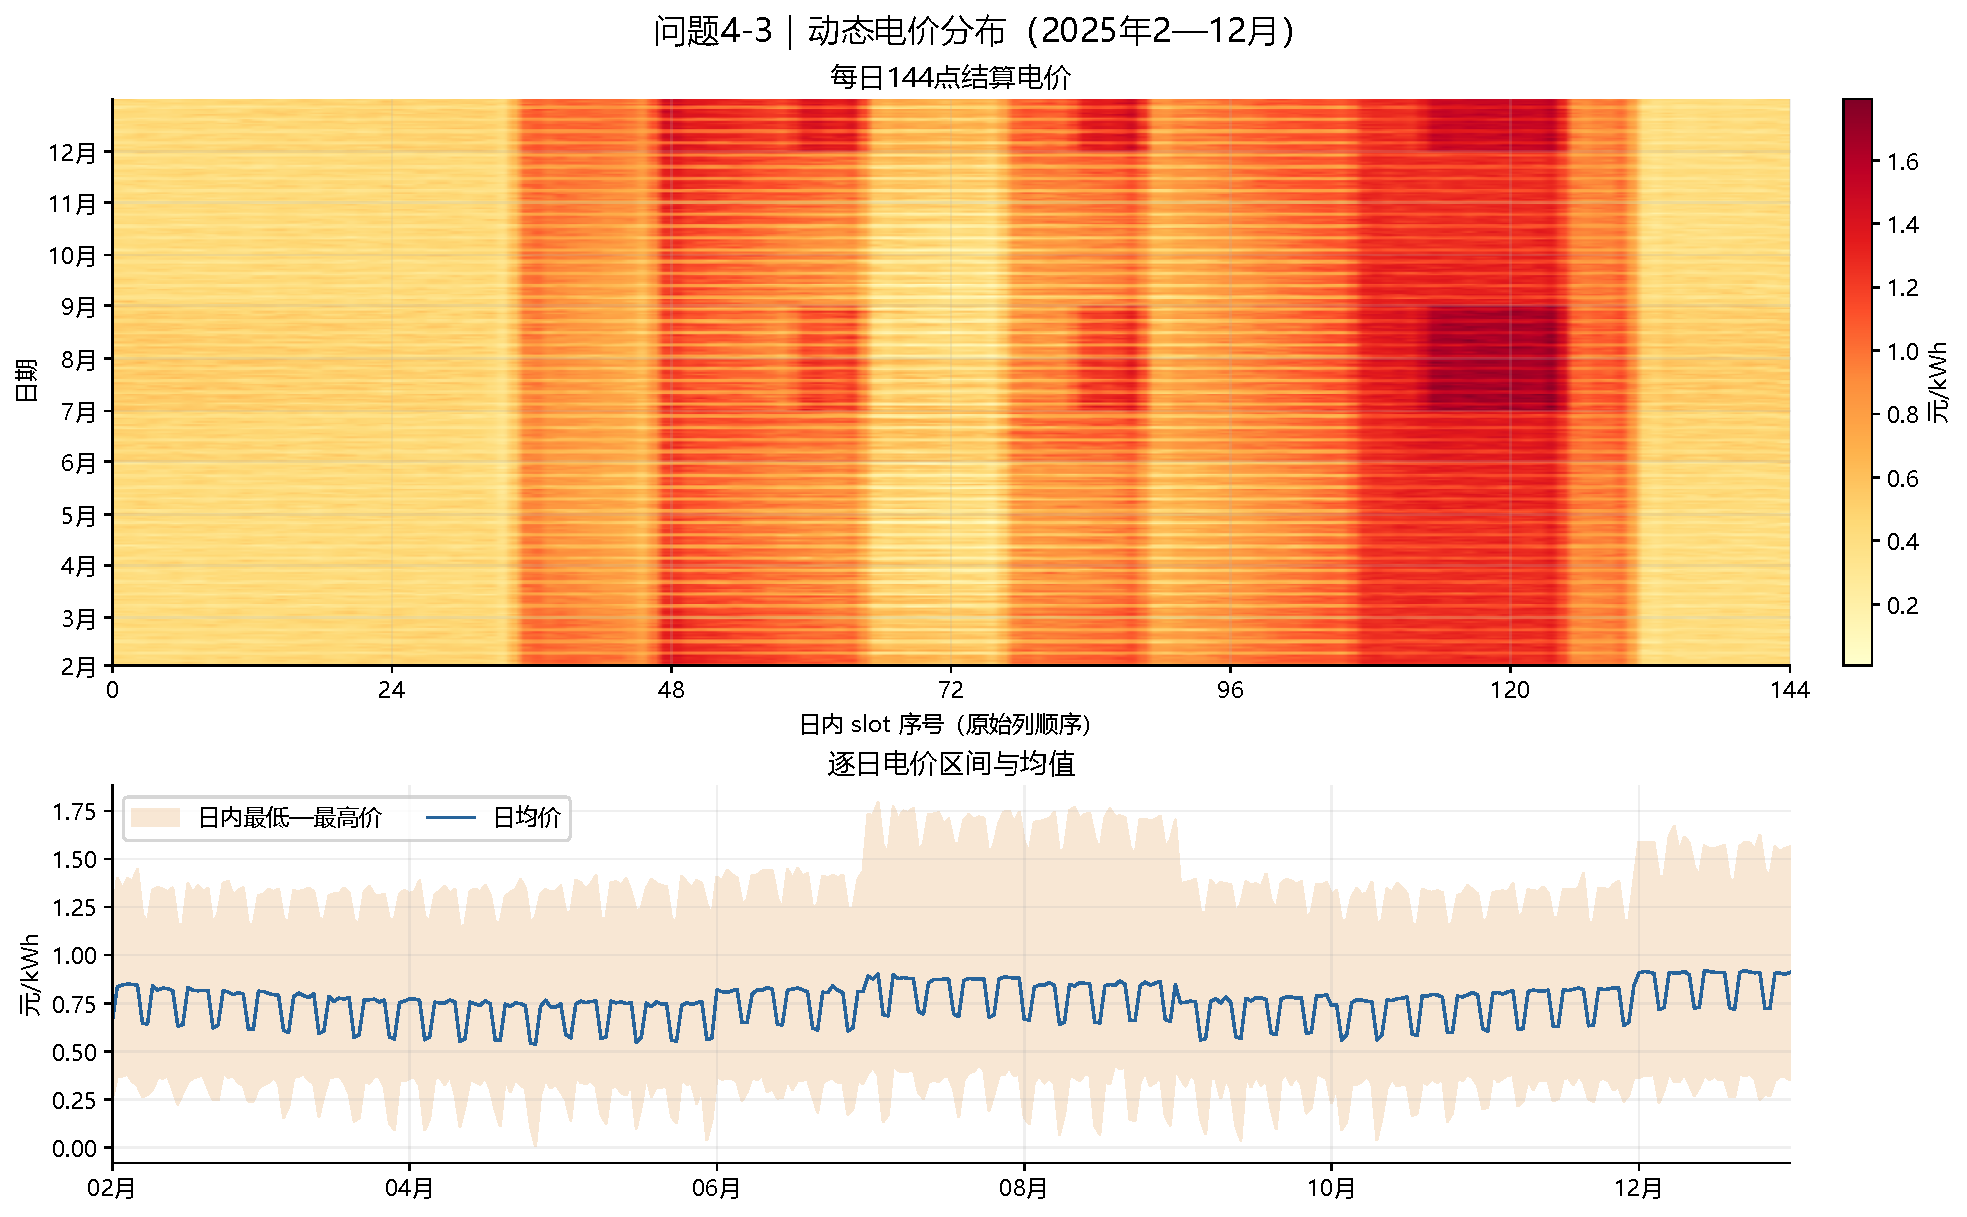
\includegraphics[width=.94\textwidth]{figures/q4_prices.pdf}
\caption{附件4的动态价格分布与日内波动特征}\end{figure}
4-3中价格峰谷差与储能吞吐量的描述性相关系数为-0.0299，未显示明显正相关。因此不能将“峰谷差越大必然充放电越多”写成当前数据结论。相关统计也不构成价格波动影响的因果识别。
\subsection{指定日期结果}
所有电量单位为kWh，费用单位为元，保留四位小数，总量使用未舍入值计算。指定十分钟区间按模板标签查询，时间口径见前文。
\Needspace{140pt}\begingroup\centering\captionof{table}{问题4-2：指定时段购电及全天合同费用}\fontsize{9}{11}\selectfont\setlength{\tabcolsep}{2pt}\renewcommand{\arraystretch}{1.13}
\noindent\begin{minipage}{\textwidth}\centering\textbf{2025-03-20}\par\smallskip
\begin{tabularx}{\textwidth}{|Y|Y|Y|Y|Y|Y|}\hline 时间段&购电量&时间段&购电量&时间段&购电量\\\hline
10:00-10:10 & 0.0000 & 12:00-12:10 & 671.0825 & 14:00-14:10 & 0.0000\\\hline
16:00-16:10 & 545.0921 & 18:00-18:10 & 715.8517 & 20:00-20:10 & 729.7183\\\hline
\multicolumn{2}{|c|}{全天合同购电量}&76140.7317&\multicolumn{2}{c|}{全天合同购电费}&47497.6864\\\hline\end{tabularx}\end{minipage}\par\medskip
\noindent\begin{minipage}{\textwidth}\centering\textbf{2025-06-21}\par\smallskip
\begin{tabularx}{\textwidth}{|Y|Y|Y|Y|Y|Y|}\hline 时间段&购电量&时间段&购电量&时间段&购电量\\\hline
10:00-10:10 & 0.0000 & 12:00-12:10 & 735.1763 & 14:00-14:10 & 0.0000\\\hline
16:00-16:10 & 524.8433 & 18:00-18:10 & 701.5525 & 20:00-20:10 & 888.2017\\\hline
\multicolumn{2}{|c|}{全天合同购电量}&77616.4592&\multicolumn{2}{c|}{全天合同购电费}&38449.1099\\\hline\end{tabularx}\end{minipage}\par\medskip
\noindent\begin{minipage}{\textwidth}\centering\textbf{2025-09-23}\par\smallskip
\begin{tabularx}{\textwidth}{|Y|Y|Y|Y|Y|Y|}\hline 时间段&购电量&时间段&购电量&时间段&购电量\\\hline
10:00-10:10 & 0.0000 & 12:00-12:10 & 494.2704 & 14:00-14:10 & 0.0000\\\hline
16:00-16:10 & 457.1233 & 18:00-18:10 & 802.0687 & 20:00-20:10 & 508.3743\\\hline
\multicolumn{2}{|c|}{全天合同购电量}&68909.8634&\multicolumn{2}{c|}{全天合同购电费}&44029.5706\\\hline\end{tabularx}\end{minipage}\par\medskip
\noindent\begin{minipage}{\textwidth}\centering\textbf{2025-12-21}\par\smallskip
\begin{tabularx}{\textwidth}{|Y|Y|Y|Y|Y|Y|}\hline 时间段&购电量&时间段&购电量&时间段&购电量\\\hline
10:00-10:10 & 0.0000 & 12:00-12:10 & 910.9646 & 14:00-14:10 & 0.0000\\\hline
16:00-16:10 & 778.8025 & 18:00-18:10 & 727.5967 & 20:00-20:10 & 0.0000\\\hline
\multicolumn{2}{|c|}{全天合同购电量}&93437.8248&\multicolumn{2}{c|}{全天合同购电费}&69304.3080\\\hline\end{tabularx}\end{minipage}\par\medskip
\raggedright 注：购电量为日前计划，合同费用不含紧急购电费。\par\endgroup\medskip
\Needspace{140pt}\begingroup\centering\captionof{table}{问题4-2：指定时段储能充放电及首末储电量}\fontsize{9}{11}\selectfont\setlength{\tabcolsep}{2pt}\renewcommand{\arraystretch}{1.12}
\noindent\begin{minipage}{\textwidth}\centering\textbf{2025-03-20}\par\smallskip\begin{tabularx}{\textwidth}{|Y|Y|Y|Y|Y|Y|}\hline 时间段&充电量&放电量&时间段&充电量&放电量\\\hline
0:00-4:00 & 2000.0000 & 0.0000 & 4:00-8:00 & 4166.6667 & 4772.4051\\\hline
8:00-12:00 & 5850.7628 & 4542.5949 & 12:00-16:00 & 5919.3802 & 893.8158\\\hline
16:00-20:00 & 0.0000 & 6442.3836 & 20:00-24:00 & 5333.3333 & 2197.6164\\\hline
\multicolumn{2}{|c|}{0:00储电量}&6000.0000&\multicolumn{2}{c|}{24:00储电量}&6000.0000\\\hline\end{tabularx}\end{minipage}\par\medskip
\noindent\begin{minipage}{\textwidth}\centering\textbf{2025-06-21}\par\smallskip\begin{tabularx}{\textwidth}{|Y|Y|Y|Y|Y|Y|}\hline 时间段&充电量&放电量&时间段&充电量&放电量\\\hline
0:00-4:00 & 833.3333 & 1345.2267 & 4:00-8:00 & 6204.7848 & 4974.9353\\\hline
8:00-12:00 & 5866.5994 & 3187.6593 & 12:00-16:00 & 6129.3106 & 1589.7416\\\hline
16:00-20:00 & 0.0000 & 5810.8187 & 20:00-24:00 & 5333.3333 & 2829.1812\\\hline
\multicolumn{2}{|c|}{0:00储电量}&6000.0000&\multicolumn{2}{c|}{24:00储电量}&6000.0000\\\hline\end{tabularx}\end{minipage}\par\medskip
\noindent\begin{minipage}{\textwidth}\centering\textbf{2025-09-23}\par\smallskip\begin{tabularx}{\textwidth}{|Y|Y|Y|Y|Y|Y|}\hline 时间段&充电量&放电量&时间段&充电量&放电量\\\hline
0:00-4:00 & 2833.3333 & 0.0000 & 4:00-8:00 & 2500.0000 & 6584.5173\\\hline
8:00-12:00 & 5484.0361 & 2055.4827 & 12:00-16:00 & 5442.4853 & 210.4823\\\hline
16:00-20:00 & 0.0000 & 6973.3333 & 20:00-24:00 & 5333.3333 & 1666.6667\\\hline
\multicolumn{2}{|c|}{0:00储电量}&6000.0000&\multicolumn{2}{c|}{24:00储电量}&6000.0000\\\hline\end{tabularx}\end{minipage}\par\medskip
\noindent\begin{minipage}{\textwidth}\centering\textbf{2025-12-21}\par\smallskip\begin{tabularx}{\textwidth}{|Y|Y|Y|Y|Y|Y|}\hline 时间段&充电量&放电量&时间段&充电量&放电量\\\hline
0:00-4:00 & 5333.3333 & 0.0000 & 4:00-8:00 & 833.3333 & 1508.3333\\\hline
8:00-12:00 & 5833.3333 & 7806.6667 & 12:00-16:00 & 7500.0000 & 2315.3528\\\hline
16:00-20:00 & 191.7936 & 5131.2538 & 20:00-24:00 & 5333.3333 & 3508.7462\\\hline
\multicolumn{2}{|c|}{0:00储电量}&6000.0000&\multicolumn{2}{c|}{24:00储电量}&6000.0000\\\hline\end{tabularx}\end{minipage}\par\medskip
\raggedright 注：四小时内充放电均为正表示不同十分钟时段的累计，不表示同时充放电。\par\endgroup
\begin{table}[H]\centering\caption{问题4-2：四个指定日期的紧急购电区间}\label{tab:emergency-问题4-2}\fontsize{9}{11}\selectfont\setlength{\tabcolsep}{2pt}\begin{tabular}{|lr|lr|lr|lr|}\hline
\multicolumn{2}{|c|}{2025-03-20} & \multicolumn{2}{|c|}{2025-06-21} & \multicolumn{2}{|c|}{2025-09-23} & \multicolumn{2}{|c|}{2025-12-21}\\\hline
时间段&购电量&时间段&购电量&时间段&购电量&时间段&购电量\\\hline
0:30-0:50 & 37.4563 & 无 & 0.0000 & 2:10-2:20 & 0.8426 & 0:10-0:20 & 3.3265\\
1:20-1:30 & 11.5129 &  &  & 6:10-8:10 & 490.6818 & 1:10-1:30 & 22.4663\\
18:10-18:30 & 8.8068 &  &  & 8:30-8:40 & 6.7917 & 1:40-1:50 & 1.5754\\
18:50-19:20 & 68.9363 &  &  & 9:30-11:20 & 520.6356 & 2:20-2:30 & 6.5004\\
20:10-20:30 & 53.6129 &  &  & 14:30-15:40 & 382.7140 & 3:10-3:30 & 59.6043\\
21:30-21:40 & 8.8117 &  &  & 16:00-18:00 & 370.6423 & 3:40-4:00 & 98.1948\\
23:40-23:50 & 24.6080 &  &  & 20:20-20:40 & 7.5098 & 4:20-4:30 & 0.1398\\
 &  &  &  & 21:00-21:10 & 9.3900 & 5:10-5:30 & 9.6256\\
 &  &  &  & 22:30-22:40 & 16.1867 & 5:40-6:10 & 47.7728\\
 &  &  &  &  &  & 6:20-6:40 & 25.1715\\
 &  &  &  &  &  & 7:0-7:20 & 10.0867\\
 &  &  &  &  &  & 7:50-8:10 & 24.5775\\
 &  &  &  &  &  & 8:30-8:50 & 39.6960\\
 &  &  &  &  &  & 9:00-9:20 & 26.6807\\
 &  &  &  &  &  & 9:40-10:00 & 33.1458\\
 &  &  &  &  &  & 10:30-12:00 & 1038.4861\\
 &  &  &  &  &  & 12:10-12:30 & 25.4431\\
 &  &  &  &  &  & 12:40-13:30 & 166.5758\\
 &  &  &  &  &  & 14:50-16:10 & 179.9651\\
 &  &  &  &  &  & 16:30-16:40 & 9.4271\\
 &  &  &  &  &  & 17:30-17:40 & 17.9450\\
 &  &  &  &  &  & 18:20-18:30 & 6.9191\\
 &  &  &  &  &  & 18:40-19:10 & 29.1800\\
 &  &  &  &  &  & 19:30-19:40 & 1.0733\\
 &  &  &  &  &  & 19:50-20:20 & 69.4854\\
 &  &  &  &  &  & 22:00-22:10 & 15.0150\\
 &  &  &  &  &  & 23:00-23:20 & 15.7499\\
 &  &  &  &  &  & 23:50-0:00+1 & 6.6598\\
\hline\end{tabular}\end{table}

\begin{table}[H]\centering\small
\caption{问题4-2：实际总购电与费用}
\begin{tabular}{lrrrr}\toprule
日期 & 实际购电量 & 紧急购电量 & 紧急费用 & 实际总费用\\\midrule
2025-03-20 & 76354.4766 & 213.7449 & 1045.3672 & 48543.0536\\
2025-06-21 & 77616.4592 & 0.0000 & 0.0000 & 38449.1099\\
2025-09-23 & 70715.2578 & 1805.3944 & 7981.0571 & 52010.6277\\
2025-12-21 & 95428.3138 & 1990.4890 & 9118.8195 & 78423.1274\\
\bottomrule\end{tabular}\end{table}
\FloatBarrier
\subsection{指定日期结果}
所有电量单位为kWh，费用单位为元，保留四位小数，总量使用未舍入值计算。指定十分钟区间按模板标签查询，时间口径见前文。
\Needspace{140pt}\begingroup\centering\captionof{table}{问题4-3：指定时段购电及全天合同费用}\fontsize{9}{11}\selectfont\setlength{\tabcolsep}{2pt}\renewcommand{\arraystretch}{1.13}
\noindent\begin{minipage}{\textwidth}\centering\textbf{2025-03-20}\par\smallskip
\begin{tabularx}{\textwidth}{|Y|Y|Y|Y|Y|Y|}\hline 时间段&购电量&时间段&购电量&时间段&购电量\\\hline
10:00-10:10 & \shortstack{0.0000\\0.0000} & 12:00-12:10 & \shortstack{599.0619\\521.3555} & 14:00-14:10 & \shortstack{0.0000\\0.0000}\\\hline
16:00-16:10 & \shortstack{646.6018\\493.7743} & 18:00-18:10 & \shortstack{711.7617\\711.7617} & 20:00-20:10 & \shortstack{729.7183\\729.7183}\\\hline
\multicolumn{2}{|c|}{全天合同购电量}&\shortstack{73540.3073\\68104.3475}&\multicolumn{2}{c|}{全天合同购电费}&\shortstack{45498.3173\\44219.9049}\\\hline\end{tabularx}\end{minipage}\par\medskip
\noindent\begin{minipage}{\textwidth}\centering\textbf{2025-06-21}\par\smallskip
\begin{tabularx}{\textwidth}{|Y|Y|Y|Y|Y|Y|}\hline 时间段&购电量&时间段&购电量&时间段&购电量\\\hline
10:00-10:10 & \shortstack{0.0000\\0.0000} & 12:00-12:10 & \shortstack{561.4173\\561.4173} & 14:00-14:10 & \shortstack{0.0000\\0.0000}\\\hline
16:00-16:10 & \shortstack{575.5241\\575.5241} & 18:00-18:10 & \shortstack{686.7649\\686.7649} & 20:00-20:10 & \shortstack{888.2017\\888.2017}\\\hline
\multicolumn{2}{|c|}{全天合同购电量}&\shortstack{74926.2075\\74783.7930}&\multicolumn{2}{c|}{全天合同购电费}&\shortstack{37486.1181\\37518.1788}\\\hline\end{tabularx}\end{minipage}\par\medskip
\noindent\begin{minipage}{\textwidth}\centering\textbf{2025-09-23}\par\smallskip
\begin{tabularx}{\textwidth}{|Y|Y|Y|Y|Y|Y|}\hline 时间段&购电量&时间段&购电量&时间段&购电量\\\hline
10:00-10:10 & \shortstack{0.0000\\0.0000} & 12:00-12:10 & \shortstack{445.1351\\430.5782} & 14:00-14:10 & \shortstack{23.4920\\0.0000}\\\hline
16:00-16:10 & \shortstack{600.6055\\563.8344} & 18:00-18:10 & \shortstack{833.5750\\833.5750} & 20:00-20:10 & \shortstack{519.1183\\519.1183}\\\hline
\multicolumn{2}{|c|}{全天合同购电量}&\shortstack{76310.5609\\74782.7314}&\multicolumn{2}{c|}{全天合同购电费}&\shortstack{49557.9160\\49078.6917}\\\hline\end{tabularx}\end{minipage}\par\medskip
\noindent\begin{minipage}{\textwidth}\centering\textbf{2025-12-21}\par\smallskip
\begin{tabularx}{\textwidth}{|Y|Y|Y|Y|Y|Y|}\hline 时间段&购电量&时间段&购电量&时间段&购电量\\\hline
10:00-10:10 & \shortstack{0.0000\\0.0000} & 12:00-12:10 & \shortstack{972.1554\\866.2299} & 14:00-14:10 & \shortstack{0.0000\\0.0000}\\\hline
16:00-16:10 & \shortstack{825.5984\\825.5984} & 18:00-18:10 & \shortstack{727.5967\\727.5967} & 20:00-20:10 & \shortstack{0.0000\\0.0000}\\\hline
\multicolumn{2}{|c|}{全天合同购电量}&\shortstack{95616.1888\\94807.1114}&\multicolumn{2}{c|}{全天合同购电费}&\shortstack{71384.8537\\71267.4193}\\\hline\end{tabularx}\end{minipage}\par\medskip
\raggedright 注：每格上行为0:00计划，下行为执行合同；下行合同费用为初始计划费加逐次调整净费。\par\endgroup\medskip
\Needspace{140pt}\begingroup\centering\captionof{table}{问题4-3：指定时段储能充放电及首末储电量}\fontsize{9}{11}\selectfont\setlength{\tabcolsep}{2pt}\renewcommand{\arraystretch}{1.12}
\noindent\begin{minipage}{\textwidth}\centering\textbf{2025-03-20}\par\smallskip\begin{tabularx}{\textwidth}{|Y|Y|Y|Y|Y|Y|}\hline 时间段&充电量&放电量&时间段&充电量&放电量\\\hline
0:00-4:00 & 2000.0000 & 0.0000 & 4:00-8:00 & 3333.3333 & 6001.7220\\\hline
8:00-12:00 & 5493.2105 & 2638.2780 & 12:00-16:00 & 5469.1180 & 244.7150\\\hline
16:00-20:00 & 21.2974 & 6454.7379 & 20:00-24:00 & 5333.3333 & 2197.2840\\\hline
\multicolumn{2}{|c|}{0:00储电量}&6000.0000&\multicolumn{2}{c|}{24:00储电量}&6000.0000\\\hline\end{tabularx}\end{minipage}\par\medskip
\noindent\begin{minipage}{\textwidth}\centering\textbf{2025-06-21}\par\smallskip\begin{tabularx}{\textwidth}{|Y|Y|Y|Y|Y|Y|}\hline 时间段&充电量&放电量&时间段&充电量&放电量\\\hline
0:00-4:00 & 833.3333 & 1345.2267 & 4:00-8:00 & 6301.4782 & 4835.8011\\\hline
8:00-12:00 & 5668.5263 & 3272.8270 & 12:00-16:00 & 5611.2061 & 1300.5077\\\hline
16:00-20:00 & 195.7802 & 5823.2065 & 20:00-24:00 & 5333.3333 & 2816.7935\\\hline
\multicolumn{2}{|c|}{0:00储电量}&6000.0000&\multicolumn{2}{c|}{24:00储电量}&6000.0000\\\hline\end{tabularx}\end{minipage}\par\medskip
\noindent\begin{minipage}{\textwidth}\centering\textbf{2025-09-23}\par\smallskip\begin{tabularx}{\textwidth}{|Y|Y|Y|Y|Y|Y|}\hline 时间段&充电量&放电量&时间段&充电量&放电量\\\hline
0:00-4:00 & 2833.3333 & 0.0000 & 4:00-8:00 & 2500.0000 & 6097.8774\\\hline
8:00-12:00 & 5893.1650 & 2517.5563 & 12:00-16:00 & 5663.8446 & 745.7440\\\hline
16:00-20:00 & 7.0598 & 6979.0518 & 20:00-24:00 & 5333.3333 & 1666.6667\\\hline
\multicolumn{2}{|c|}{0:00储电量}&6000.0000&\multicolumn{2}{c|}{24:00储电量}&6000.0000\\\hline\end{tabularx}\end{minipage}\par\medskip
\noindent\begin{minipage}{\textwidth}\centering\textbf{2025-12-21}\par\smallskip\begin{tabularx}{\textwidth}{|Y|Y|Y|Y|Y|Y|}\hline 时间段&充电量&放电量&时间段&充电量&放电量\\\hline
0:00-4:00 & 5333.3333 & 0.0000 & 4:00-8:00 & 833.3333 & 1656.5123\\\hline
8:00-12:00 & 5833.3333 & 7403.0251 & 12:00-16:00 & 7365.6197 & 2633.6307\\\hline
16:00-20:00 & 356.2915 & 5118.8381 & 20:00-24:00 & 5333.3333 & 3482.7419\\\hline
\multicolumn{2}{|c|}{0:00储电量}&6000.0000&\multicolumn{2}{c|}{24:00储电量}&6000.0000\\\hline\end{tabularx}\end{minipage}\par\medskip
\raggedright 注：四小时内充放电均为正表示不同十分钟时段的累计，不表示同时充放电。\par\endgroup
\begin{table}[H]\centering\caption{问题4-3：四个指定日期的紧急购电区间}\label{tab:emergency-问题4-3}\fontsize{9}{11}\selectfont\setlength{\tabcolsep}{2pt}\begin{tabular}{|lr|lr|lr|lr|}\hline
\multicolumn{2}{|c|}{2025-03-20} & \multicolumn{2}{|c|}{2025-06-21} & \multicolumn{2}{|c|}{2025-09-23} & \multicolumn{2}{|c|}{2025-12-21}\\\hline
时间段&购电量&时间段&购电量&时间段&购电量&时间段&购电量\\\hline
0:30-0:50 & 37.4563 & 无 & 0.0000 & 2:10-2:20 & 0.8426 & 0:10-0:20 & 3.3265\\
1:20-1:30 & 11.5129 &  &  & 20:20-20:40 & 7.5098 & 1:10-1:30 & 22.4663\\
8:20-8:40 & 28.2239 &  &  & 21:00-21:10 & 9.3900 & 1:40-1:50 & 1.5754\\
8:50-9:30 & 137.5983 &  &  & 22:30-22:40 & 16.1867 & 2:20-2:30 & 6.5004\\
9:50-10:10 & 57.9445 &  &  &  &  & 3:10-3:30 & 59.6043\\
11:10-12:10 & 345.6128 &  &  &  &  & 3:40-4:00 & 98.1948\\
12:40-13:00 & 150.4760 &  &  &  &  & 4:20-4:30 & 0.1398\\
13:10-13:50 & 148.0535 &  &  &  &  & 5:10-5:30 & 9.6256\\
14:00-14:40 & 40.9799 &  &  &  &  & 5:40-6:10 & 47.7728\\
15:30-16:30 & 93.3849 &  &  &  &  & 6:30-6:40 & 0.4267\\
16:40-17:00 & 5.1731 &  &  &  &  & 8:00-8:10 & 13.3395\\
18:10-18:30 & 8.8068 &  &  &  &  & 8:30-8:40 & 6.0161\\
18:50-19:20 & 71.7835 &  &  &  &  & 9:00-9:10 & 0.7455\\
20:10-20:30 & 53.6129 &  &  &  &  & 9:40-10:10 & 57.1657\\
21:30-21:40 & 8.8117 &  &  &  &  & 10:30-10:40 & 30.1744\\
23:40-23:50 & 24.6080 &  &  &  &  & 10:50-12:30 & 651.1456\\
 &  &  &  &  &  & 12:50-13:20 & 99.6146\\
 &  &  &  &  &  & 17:30-17:40 & 17.9450\\
 &  &  &  &  &  & 18:20-18:30 & 6.9191\\
 &  &  &  &  &  & 18:40-19:10 & 30.7700\\
 &  &  &  &  &  & 19:30-19:40 & 2.4650\\
 &  &  &  &  &  & 19:50-20:20 & 84.0870\\
 &  &  &  &  &  & 22:00-22:10 & 15.0150\\
 &  &  &  &  &  & 23:00-23:20 & 15.7499\\
 &  &  &  &  &  & 23:50-0:00+1 & 6.6598\\
\hline\end{tabular}\end{table}

\begin{table}[H]\centering\small
\caption{问题4-3：实际总购电与费用}
\begin{tabular}{lrrrr}\toprule
日期 & 实际购电量 & 紧急购电量 & 紧急费用 & 实际总费用\\\midrule
2025-03-20 & 69328.3866 & 1224.0390 & 4936.1720 & 49156.0769\\
2025-06-21 & 74783.7930 & 0.0000 & 0.0000 & 37518.1788\\
2025-09-23 & 74816.6604 & 33.9290 & 139.0167 & 49217.7084\\
2025-12-21 & 96094.5564 & 1287.4449 & 5561.4233 & 76828.8427\\
\bottomrule\end{tabular}\end{table}
\FloatBarrier

\begin{figure}[H]\centering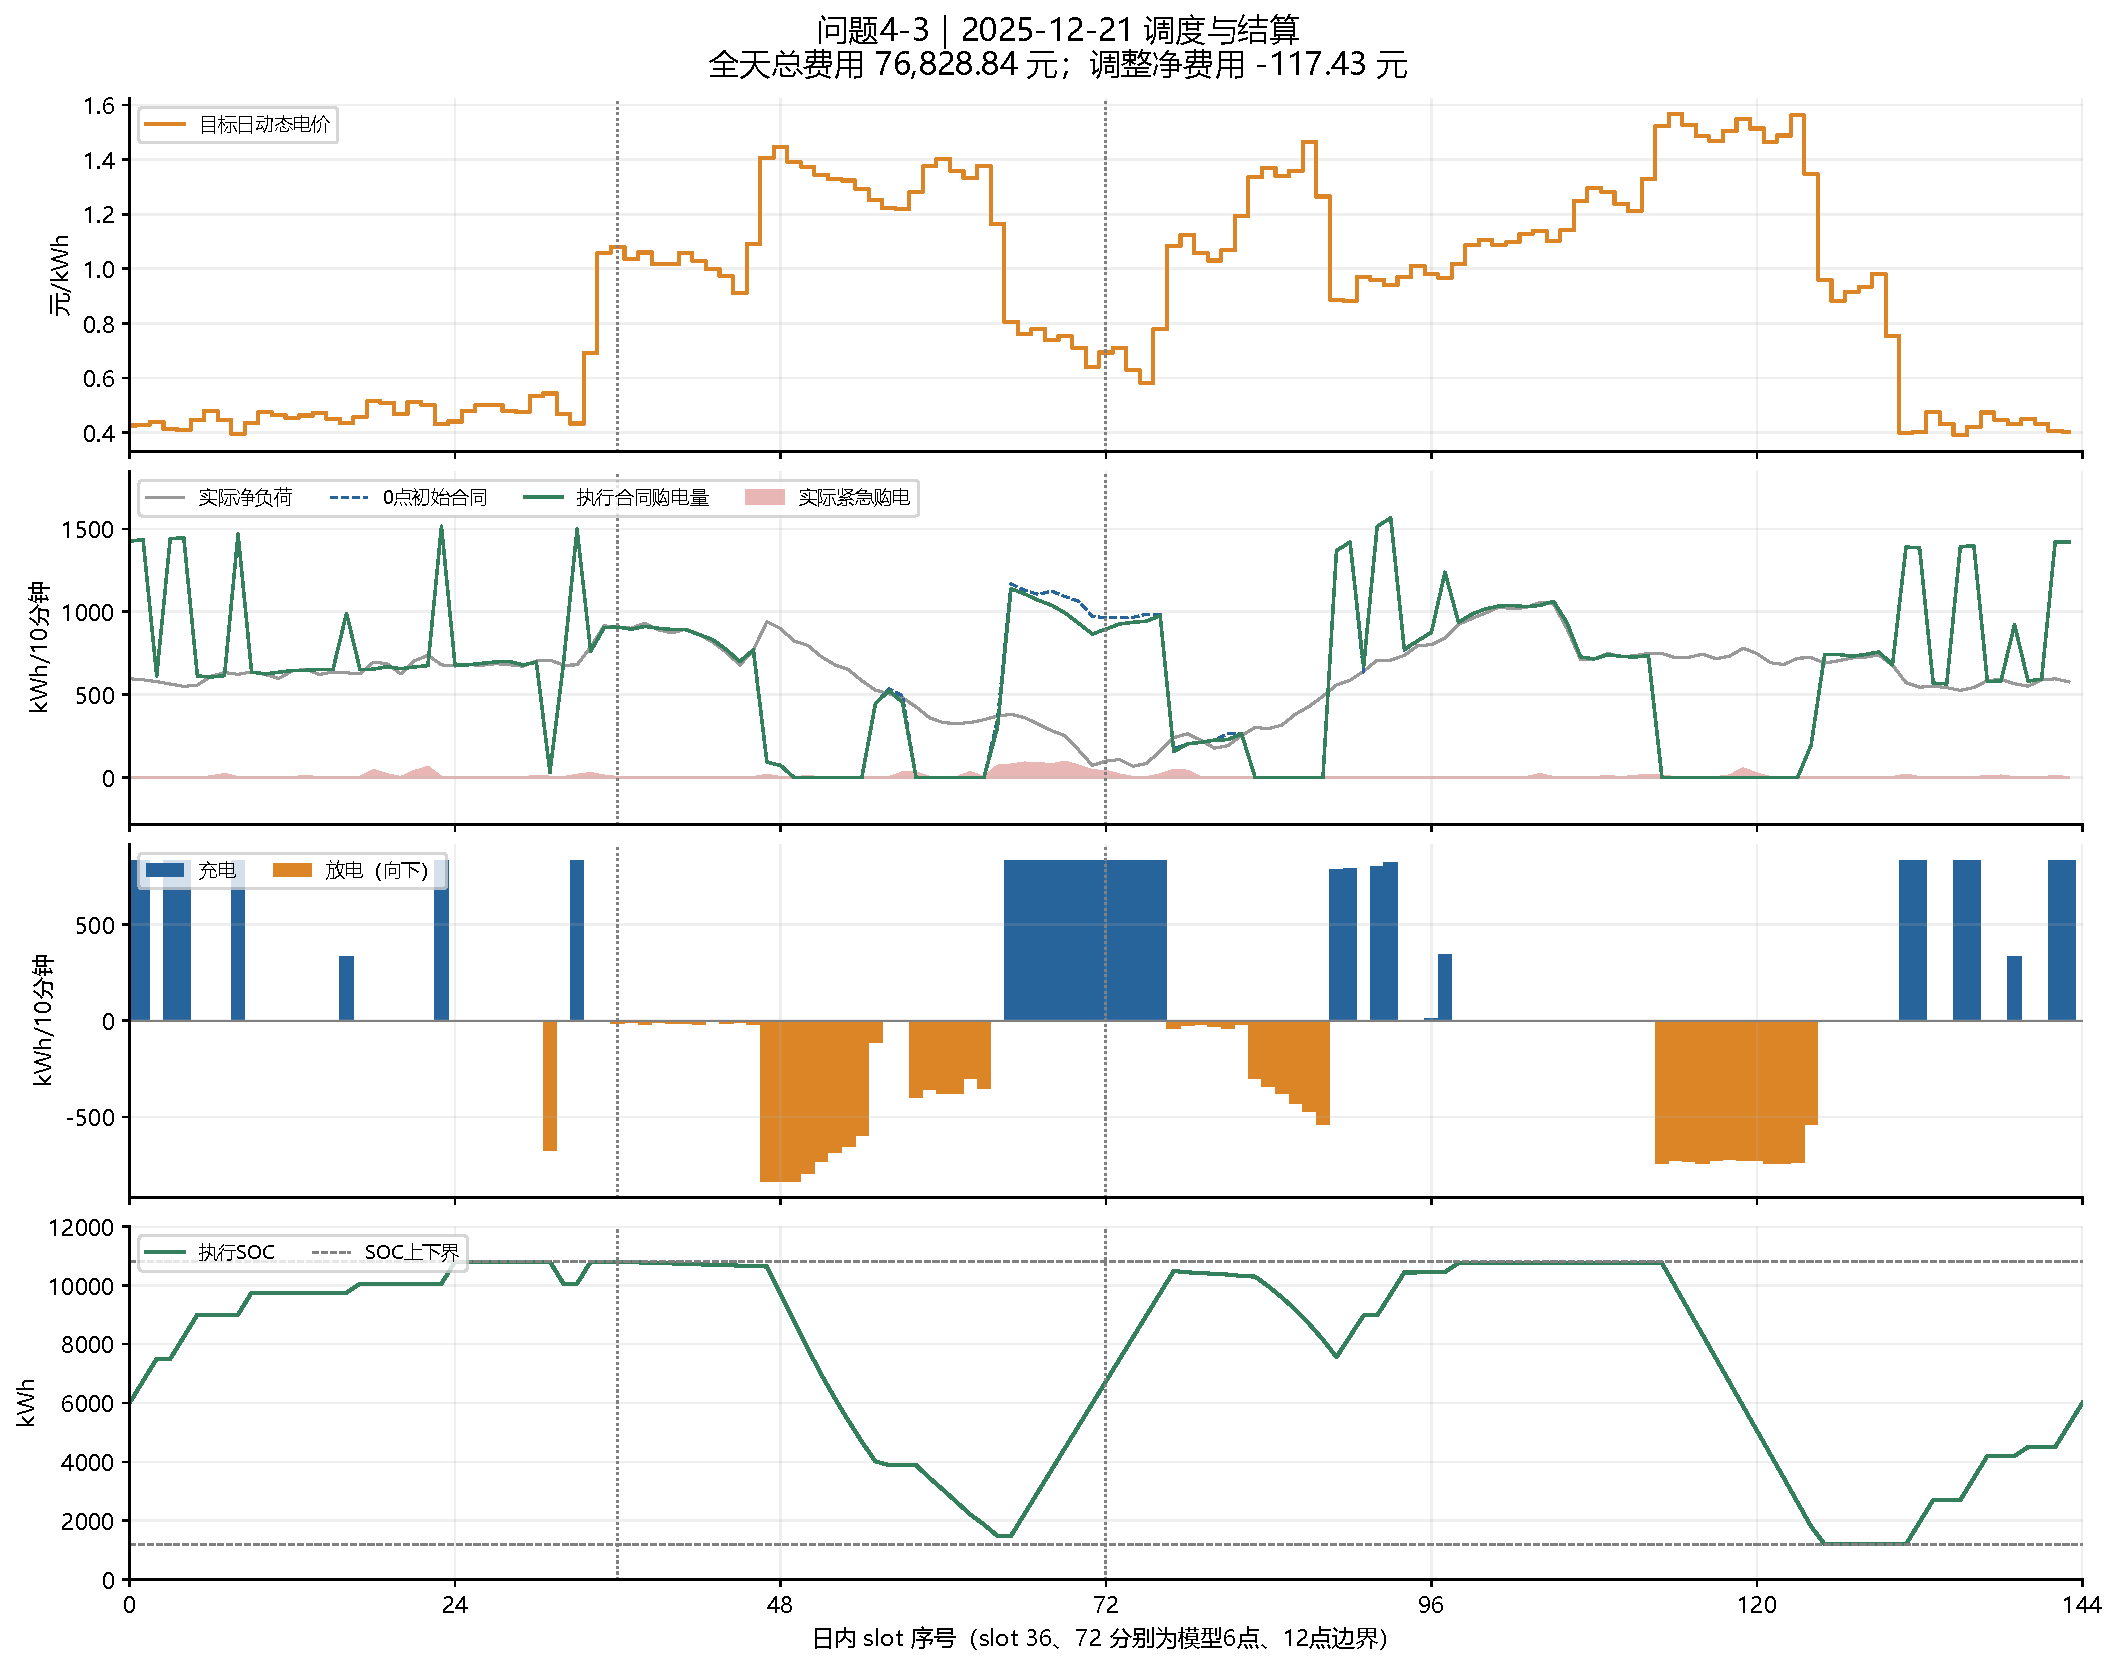
\includegraphics[width=.94\textwidth]{figures/q4_dispatch.pdf}
\caption{波动价格下12月21日的滚动合同与储能执行策略}\end{figure}
\FloatBarrier

\section{算法对照、敏感性与模型检验}
\subsection{同信息日前方法与滚动信息价值}
在相同334天、设备参数和固定电价下，DET使用前31天净负荷均值，Q80使用逐段80\%分位数，二者均调用确定性储能LP；SAA直接使用问题二，CVaR在同一历史场景上引入紧急费用尾部惩罚。上述四者在0:00拥有相同历史信息。SAA-MPC使用问题三的已发布光伏预报及日内更新，因此在表中单列为信息与机制拓展，不能用其差异证明纯算法优势。

\begin{table}[H]\centering\small
\caption{预设主方法的费用与风险比较}
\begin{tabular}{lrrrr}\toprule
方法 & 总费用/万元 & 紧急电量/万kWh & 紧急天数 & 日费CVaR95/元\\\midrule
DET & 2507.3342 & 325.7900 & 287 & 141532.0334\\
Q80 & 1773.5842 & 53.7269 & 249 & 85423.1426\\
SAA & 1760.9792 & 47.7446 & 249 & 82240.4284\\
CVaR95-L50 & 1765.8749 & 18.7619 & 248 & 67777.8076\\
SAA-MPC & 1702.0307 & 28.2086 & 243 & 74761.1946\\
\bottomrule\end{tabular}\end{table}
在预设静态主比较中，SAA的实际费用最低；Q80比SAA高约0.716\%，说明较高分位数虽然有经济解释，仍不能替代跨时段联合优化。DET的补购费用较大，反映均值计划难以应对非对称缺口损失。SAA-MPC比SAA降低费用约3.347\%，收益来源的进一步分解见第三问。

\subsection{CVaR风险规避与参数敏感性}
设历史场景全天紧急费用为$L_s=\sum_t5p_tU_t^{(s)}$，引入阈值$z$和超额损失$\xi_s$：
\begin{align}
\operatorname{CVaR}_{\alpha}(L)&=z+\frac{1}{1-\alpha}\sum_s\pi_s\xi_s,\\
\xi_s&\geq L_s-z,\quad\xi_s\geq0.
\end{align}
目标为计划费加$(1-\lambda)\mathbb E[L]+\lambda\operatorname{CVaR}_{\alpha}(L)$和微小吞吐惩罚；$z$不限制符号。预设主参数为$\alpha=0.95,\lambda=0.50$，$\lambda=0$退化为SAA。优化对象是紧急费用，表中的“日费CVaR95”则为执行后实际总费用的尾部统计，二者不可混淆。

主CVaR相对SAA增加总费用约0.278\%，紧急电量减少60.704\%，日费用CVaR95下降17.586\%，体现用较高合同费用换取尾部风险降低。经验日费CVaR95按最差5\%概率质量加权，334天对应16.7天，边界样本只取剩余权重。

\begin{table}[H]\centering\small
\caption{CVaR参数敏感性：334天实际运行指标}
\begin{tabular}{lrrrr}\toprule
$\alpha$ & $\lambda$ & 总费/万元 & 紧急量/万kWh & 日费CVaR95/元\\\midrule
0.9 & 0.25 & 1750.8386 & 25.9928 & 71450.2527\\
0.9 & 0.5 & 1763.1254 & 20.1984 & 69177.9534\\
0.9 & 0.75 & 1775.1993 & 15.5810 & 67314.8892\\
0.9 & 1.0 & 1781.5115 & 14.2774 & 67171.0438\\
0.95 & 0.25 & 1752.7502 & 24.8635 & 69870.0809\\
0.95 & 0.5 & 1765.8749 & 18.7619 & 67777.8076\\
0.95 & 0.75 & 1775.1993 & 15.5810 & 67314.8892\\
0.95 & 1.0 & 1781.5115 & 14.2774 & 67171.0438\\
0.99 & 0.25 & 1752.0906 & 24.4162 & 69300.1261\\
0.99 & 0.5 & 1765.8084 & 18.7440 & 67767.8871\\
0.99 & 0.75 & 1775.1339 & 15.5561 & 67266.2923\\
0.99 & 1.0 & 1781.4634 & 14.2596 & 67166.7326\\
\bottomrule\end{tabular}\end{table}
12组参数预先固定，用于展示权衡而不根据全年结果重新挑选主参数。其中存在费用低于SAA的组合，因此不能宣称SAA优于所有风险规避参数。31个等权场景下，$\alpha=0.99$的尾部不足一个完整场景，其CVaR等于样本最大损失；高置信度并不意味着拥有充分的极端事件信息。样本外实际费用也无需随风险权重单调变化。

\begin{figure}[H]\centering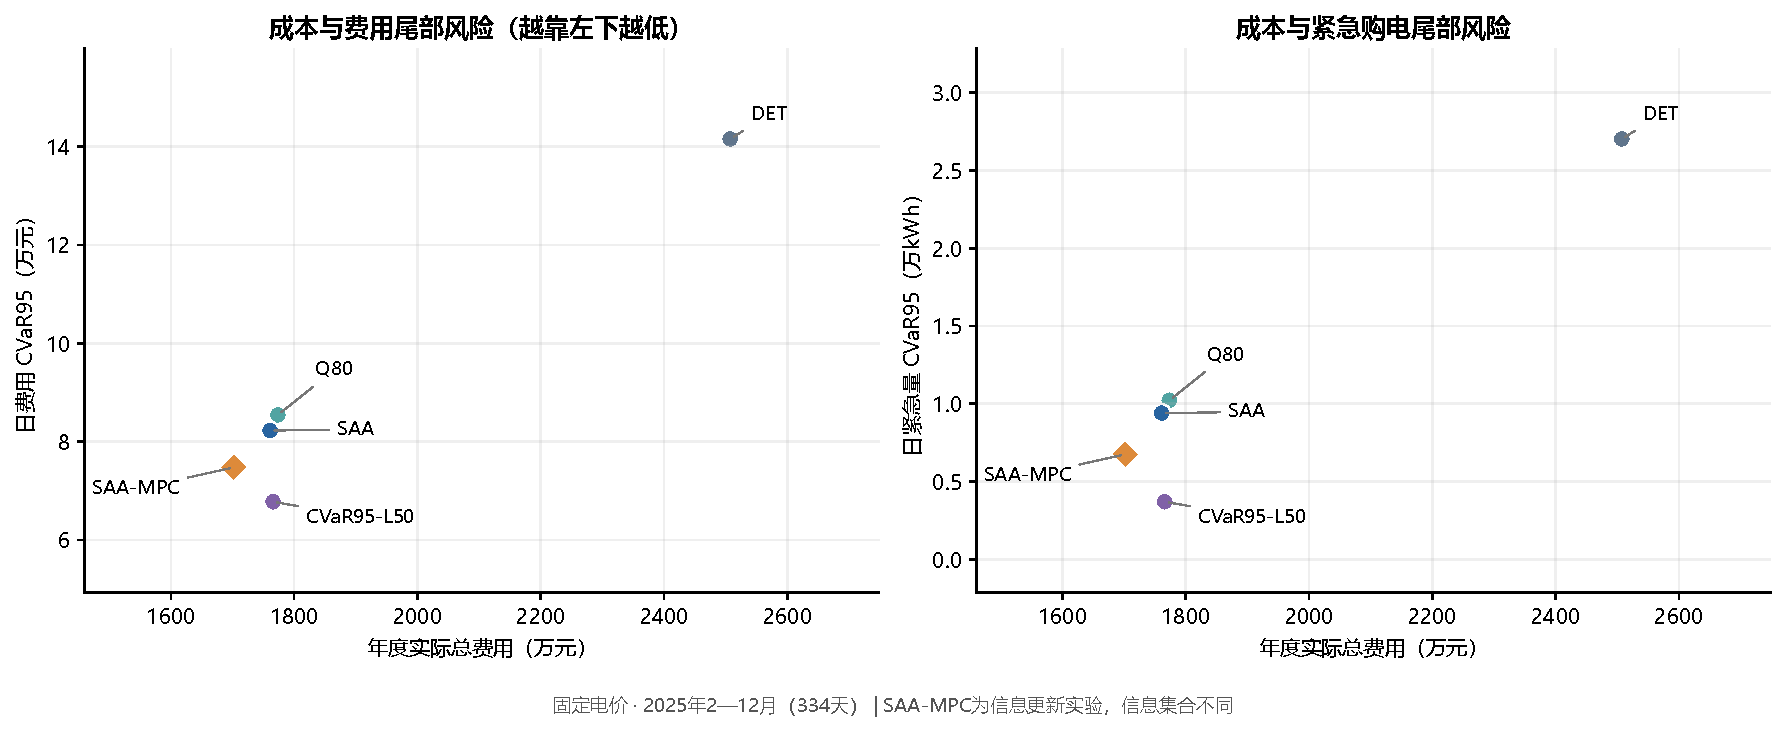
\includegraphics[width=.94\textwidth]{figures/risk_return.pdf}
\caption{预设方法的实际费用与尾部风险；MPC包含额外信息}\end{figure}
\subsection{可行性、结算与复现检验}

\begin{table}[H]\centering\small
\caption{本次合并核验的最大绝对残差（kWh）}
\begin{tabular}{lrrrr}\toprule
模型 & 供需平衡 & 储能转移 & 首末边界 & 同时充放电时段\\\midrule
Q2 & 1.14e-13 & 5.78e-12 & 0.00e+00 & 0\\
Q3 & 1.14e-13 & 1.02e-12 & 0.00e+00 & 0\\
Q4-2 & 1.14e-13 & 1.02e-12 & 0.00e+00 & 0\\
Q4-3 & 1.14e-13 & 1.02e-12 & 0.00e+00 & 0\\
\bottomrule\end{tabular}\end{table}
本次核验重算第一问和第二问334天，对第三问全期存档检查物理约束、合同恒等式及结算，并独立重算四个指定日期；第四问核对全部存档及原始价格快照。年度工作簿逐时计划、执行合同、四小时储能汇总、紧急区间与日费用均作核对。不同求解器版本可能返回等价最优解；对第二问出现差异的日期固定正式合同及四小时储能汇总重求解，核对其可行性与原最优目标，而不以新数组覆盖正式结果。

第三问19项现有测试通过，覆盖中点插值、未来实际与未发布预报隔离、执行冻结、SOC衔接、退款结算和结果导出。算法对比及12组敏感性使用归档实验结果\cite{experiment}，本次不冒称重新运行全部敏感性实验。单次运行耗时受环境影响，不作为跨硬件性能保证。

\section{模型评价与结论}
\subsection{模型优点与局限}
模型以共同线性储能约束贯穿四问，场景与真实结算分离，逐次合同调整与已执行SOC衔接清楚，便于复现及定位信息价值。正文同时给出指定日期、全期和风险对照，避免只用少量典型日支持总体结论。

局限在于：每日固定边界限制跨日调度；31天等权窗口对快速变化和尾部风险覆盖有限；未考虑电池退化、外网功率限制与未来价格预测；当前LP未显式加入互斥约束；时间标签与内部时段解释仍需最终确认。滚动求解的一系列两阶段LP不等于完整多阶段场景树，单次LP最优不代表全年实际费用全局最优。未来可引入独立验证期、季节性窗口、跨日滚动边界和电池退化成本，比较收益是否足以抵消新增复杂度。

\subsection{主要结论与运行启示}
确定性条件下，储能使示例日购电费降至35126.9486元，较无储能基准节省26.8981\%。对334天未知净负荷，SAA日前策略费用为17609791.6865元；引入光伏预报与三时刻滚动调整后为17020306.6465元，下降3.3475\%。6点与12点更新在当前回测具有明确经济收益，18点未显示额外收益。

波动电价下，4-2和4-3费用分别为17923538.0937元和17244554.4259元，同价格环境中滚动策略仍有综合经济优势。运行决策应同时关注缺口发生时刻的电价、合同富余成本与尾部风险，不能仅以平均电价、平均净负荷或最低单日费用制定策略。上述结论均限定于当前数据、价格信息假设和周期储能边界。
\FloatBarrier

\CumcmAIUsed{论文材料比较、计算口径核对、文字整合与排版。完整使用记录需由参赛队结合实际使用过程核实并随支撑材料提供}
\begin{thebibliography}{9}
\bibitem{problem} 2026年高教社杯全国大学生数学建模竞赛C题：微网与外部电网电力调控策略及附件1--5[Z]. 用户提供的赛题与数据材料, 2026.
\bibitem{experiment} CUCUM2026项目. 固定分时电价算法对比实验[Z]. 本地实验记录，评估期2025-02-01至2025-12-31, 2026.
\end{thebibliography}
\clearpage\begin{appendices}
\section{结果与复现材料索引}
本论文的正式计算来源统一位于CUCUM2026。五份结果文件均位于\path{target/}下的“附件5”目录，文件名为\path{result1.xlsx}、\path{result2.xlsx}、\path{result3.xlsx}、\path{result4-2.xlsx}和\path{result4-3.xlsx}。问题一至四求解入口分别为\path{run_question1.py}、\path{run_question2.py}、\path{run_question3.py}和\path{run_question4.py}。算法实验入口为\path{run_benchmark.py}，依赖见项目根目录\path{requirements.txt}，完整源代码位于\path{src/}。

\section{论文材料来源与核验范围}
正文图表由当前正式摘要和实验数据生成，数值快照及SHA-256见\path{paper/data_snapshot/manifest.json}。独立口径核对与逐节合并记录位于\path{paper/review/}；本次可执行核验、结果及第三问测试日志分别为\path{paper/audit_sources.py}、\path{paper/review/audit_results.json}和\path{paper/review/tests_question3.log}。PDF编译不运行优化器。

\section{初稿使用说明}
本稿用于统一论文内容和结果，学术方法参考文献、队伍完整AI使用记录及最终格式核查仍需补齐。已披露的时间标签解释及每日闭环、价格已知假设须在最终提交前确认。当前附录提供代码和结果索引，最终提交时应依适用要求补齐完整程序附录与独立支撑文件。源文件和完整工程均保留，便于后续完善。
\end{appendices}\end{document}
